\documentclass{article}
\usepackage[utf8]{inputenc}
\usepackage{pdfpages}
\input{Opsætning/Pakker}

\setcounter{secnumdepth}{4}
\setcounter{tocdepth}{4}
\usepackage[backend=biber]{biblatex}
\addbibresource{references.bib} % Erstat med stien til din .bib fil

% Definer en tilpasset kommando til at citere kun med titlen i en fodnote
\DeclareCiteCommand{\footcitetitle}[\mkbibfootnote]
  {\usebibmacro{prenote}} % Pre-note handler, her kan du indsætte information før selve citatet
  {\usebibmacro{citeindex}%
   \printtext[bibhyperref]{\mkbibbrackets{\printfield{labelnumber}}\addspace}% Tilføjer citatnummer i firkantede klammer og et mellemrum
   \printtext[bibhyperref]{\printfield{title}}} % Viser titlen efter nummeret
  {\multicitedelim} % Håndterer separator mellem flere citationer
  {\usebibmacro{postnote}} % Tilføjer post-note, bruges til at indsætte sidetal eller lignende efter citatet


\newcommand{\newchapter}{
    \cleardoublepage
    \ifthenelse{\isodd{\value{page}}}{}{\hbox{}\newpage}
}

\fancypagestyle{plain}{
    \fancyhf{}
    \renewcommand{\thepage}{\Roman{page}}
    \fancyfoot[R]{\thepage}
    \rhead{Funktionel Modellering af Matematiske Systemer i F\#}
}

\begin{document}
\begin{titlepage} % Suppresses displaying the page number on the title page and the subsequent page counts as page 1
	\newcommand{\HRule}{\rule{\linewidth}{0.5mm}} % Defines a new command for horizontal lines, change thickness here
	
	\center % Centre everything on the page
	%------------------------------------------------
	%	READ ME
	%------------------------------------------------
	   
	    %This version of the title page contains both signatures and pictures of participants, this version is best suited for larger reports and or projects. 
	
	%------------------------------------------------
	%	Headings
	%------------------------------------------------
	
	\textsc{\LARGE Danmarks Tekniske Universitet}\\[1.5cm] % Main heading such as the name of your university/college
	
    
\includegraphics[scale=0.15]{Opsætning/DTULogo.png}\\
	%\textsc{\Large Major Heading}\\[0.5cm] % Major heading such as course name
	
	%\textsc{\large Minor Heading}\\[0.5cm] % Minor heading such as course title
	
	%------------------------------------------------
	%	Title
	%------------------------------------------------
	
	\HRule\\[0.5cm]
	
	{\huge\bfseries Bachelor Projekt}\\[0.4cm] % Title of your document

	\HRule\\[0.5cm]
	%\textsc{\Large Danmarks Tekniske Universitet}\\[0.5cm] % Major heading such as course name
	
	\textsc{\Large title}\\[1cm] % Minor heading such as course title
	
	%------------------------------------------------
	%	Author(s)
	%------------------------------------------------
    \vfill\vfill\vfill
    \begin{minipage}{\textwidth}
		\begin{flushleft}
            \centering

            Jonas Dahl Larsen (s205829)
            

		\end{flushleft}
	 \end{minipage} 
    % \\[1cm]
    % \vfill \vfill
    \vspace*{1\baselineskip}


    


	%------------------------------------------------
	%	Date
	%------------------------------------------------
	
	%\vfill\vfill\vfill % Position the date 3/4 down the remaining page
	
	{\large \today} % Date, change the \today to a set date if you want to be precise
	
	\vfill % Push the date up 1/4 of the remaining page
	
\end{titlepage}
\pagenumbering{roman}
\pagestyle{plain}

\section*{Abstract}
This project aims to guide the reader through a detailed modeling of a mathematical program in F\#. By building everything from the ground up, the reader will be introduced to the basic concepts of functional programming, and how to use them to solve mathematical problems. The project aims to illustrate a strong correlation between the mathematical concepts and functional programming. Within the mathematical space, the project walks through building a number module consisting of integers, rational numbers, and complex numbers. Then, using the number module to express mathematical expressions, vectors, and matrices. Furthermore, the project will introduce the reader to property-based testing, which is used throughout the build-up to ensure the correctness of the program. The motivation behind the project is to show F\# as a possible alternative to Python in fundamental mathematical courses at Denmark's Technical University. The project concludes that using functional programming can benefit the learning process of mathematical concepts.




\newpage
\begin{figure}[h]
    \centering
    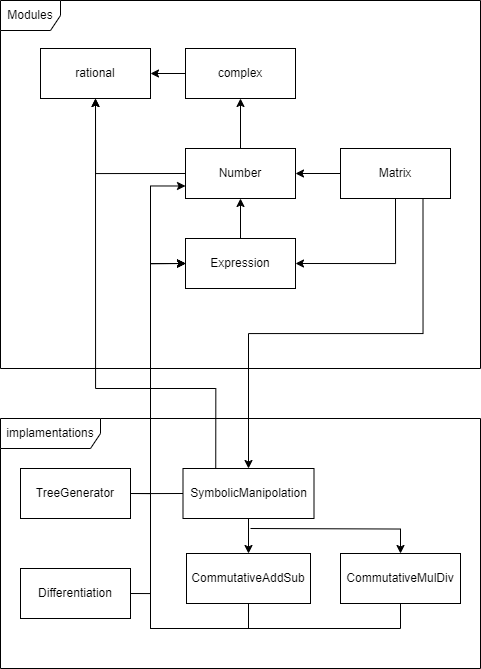
\includegraphics[width=0.8\textwidth]{Opsætning/overblik.png}
    \caption{Visuelt overblik over moduler og implementeringsfiler i programmet. $f_1 \to f_2$ indikere at $f_1$ åbner eller anvender funktioner fra $f_2$}
    \label{fig:svg_example}
\end{figure}

\newchapter
\section*{Forord}
Denne rapport er udarbejdet som et 15 ECTS bachelorprojekt i Matematik og Teknologi ved Danmarks Tekniske Universitet. Arbejdet er udført under vejledning af lektor, Ph.D. Michael Reichhardt Hansen og lektor, Ph.D. Jakob Lemvig.

Ved siden af mit studie arbejder jeg som softwareudvikler hos Secure Spectrum Fondsmæglerselskab A/S, hvor vores kodebase er skrevet i Ruby\footcitetitle{ruby}, et dynamisk typet sprog ligesom Python. Denne erfaring danner grundlag for nogle af de konklusioner, vi kommer frem til vedrørende fordelene og ulemperne mellem F\# og Python.

Programmet, som rapporten vejleder læseren igennem, kan findes på GitHub: \url{https://github.com/Larsen00/funktionsprogrammeringForIndledendeMatematik}

\newchapter
\tableofcontents
\newchapter

\pagenumbering{arabic}
\newchapter
\section{Introduktion} 

Dette projekt fokuserer på funktionel modellering af matematiske systemer ved brug af programmeringssproget F\#. I en tid, hvor programmeringssprog som Python dominerer i tekniske og videnskabelige miljøer, undersøger dette projekt fordele og ulemper ved funktionel programmering i matematiske sammenhænge. I 2023 valgte Danmarks Tekniske Universitet (DTU) at anvende Python som et hjælpeværktøj i deres grundlæggende matematik kursuser "01001 Matematik 1a" og "01002 Matematik 1b". Imidlertid åbner funktionel programmering op for et andet perspektiv og andre metoder, som kan berige og muligvis forbedre forståelsen af matematiske koncepter hos studerende.

Projektet har til formål at demonstrere, hvordan funktionel programmering, specifikt gennem F\#, kan anvendes til at opbygge og manipulere matematiske udtryk og systemer. Ved at introducere læserne til grundlæggende såvel som avancerede funktioner og teknikker i F\#, vil rapporten guide dem gennem opbygningen af funktionelle programmer, der kan løse matematiske problemer fra de grundlæggende matematik kurser på DTU. 

Rapporten vil først og fremmest dykke ned i konstruktionen af et specifikt modul for håndtering af symbolske matematiske udtryk og matrix manipulering, og deres anvendelser i forskellige matematiske kontekster. Projektets struktur og metodologi har til formål at give læseren en dybdegående forståelse af, hvordan funktionel programmering kan benyttes strategisk i matematiske discipliner, og hvordan det adskiller sig fra mere traditionelle imperative programmeringstilgange.

Gennem en systematisk tilgang til design og implementering af matematiske moduler vil rapporten udforske, hvordan matematiske og logiske principper kan integreres direkte i softwareudvikling gennem funktionel programmering. Dette vil ikke kun fremme en bedre forståelse af teoretiske koncepter gennem praktisk anvendelse, men også demonstrere F\#'s kapacitet og effektivitet i behandlingen af matematiske egenskaber.
 
\newchapter

\section{Fundamentale koncepter}
\subsection{Introduktion til Funktions Programmering}
Det forventes, at læseren har kendskab til programmering. Der gives derfor kun en kort beskrivelse af syntaks og notation, så læsere, der ikke er bekendt med F\#, kan forstå de eksempler, der løbende vil forekomme i rapporten. Vi begynder derfor med at betragte funktionen for fakultet Ligning \eqref{Fakultet}.

\begin{equation}
    \label{Fakultet}
    f(n) = \begin{cases} 
            1 &  n = 0  \\
            n \cdot f(n-1) & n > 0 \\
            \text{undefined} & n < 0 
           \end{cases}
\end{equation}

Et eksempel på en implementering i F\# er givet i Listing \ref{lst:fsharp_factorial}, som kan sammenlignes med Python-koden i Listing \ref{lst:python_factorial}, da Python og pseudokode er næsten det samme.


\begin{lstlisting}[language={FSharp}, label={lst:fsharp_factorial}, caption={Eksempel på Fakultet i F\#}]
// Fakultet i F#
let rec factorial n =
    match n with
    | 0             -> 1 
    | x when x > 0  -> x * factorial (x - 1)
    | _             -> failwith "Negative argument"
\end{lstlisting}

\begin{lstlisting}[language={FSharp}, label={lst:python_factorial}, caption={Eksempel på Fakultet i Python}]
# Fakultet i Python
def factorial(n):
    if n == 0:
        return 1
    elif n > 0:
        return n * factorial(n - 1)
    else:
        raise ValueError("Negative argument")
\end{lstlisting}

I F\# anvendes \textcolor{blue}{let} til at definere en ny variabel eller, i dette tilfælde, en funktion kaldet \textcolor{red}{factorial}. Næste nøgleord er \textcolor{blue}{rec}, hvilket indikerer, at funktionen er rekursiv. Funktionen tager et inputargument \(n\), og i linje 3 starter et match-udtryk. Her er \(n\) vores udtryk, og efter \textcolor{codepurple}{with} begynder en række mønstre, som udtrykket forsøger at matche på, separeret med '\(\vert\)'. Resultatet af funktionen vil være den kode, der eksekveres efter '\(\rightarrow\)', på den linje, hvor mønsteret er genkendt.
    
I F\#, er det som udgangspunkt ikke nødvendigt at anvende parenteser som i andre programmeringssprog. Derfor vil de kun blive anvendt, hvor det er nødvendigt gennem rapporten, typisk i sammenhænge med kædning af funktioner. For at undgå brugen af parenteser kan man i F\# benytte pipe-operatorerne, $|>$ og $<|$, som fører resultatet fra en udledning direkte ind i den næste funktion. Nedenstående eksempel viser tre ækvivalente udtryk, der demonstrerer anvendelsen af disse operatorer.

\begin{lstlisting}[style=output, label={lst:pipe_operator}, caption={Eksempel på anvendelse af pipe-operatorer i F\# ved udregning af $(3!)! = 6! = 720 $.}]
> factorial (factorial 3);;
val it: int = 720

> factorial <| factorial 3;;
val it: int = 720

> factorial 3 |> factorial;;
val it: int = 720
\end{lstlisting}


% Et match på et mønster er ikke det samme som '==' kendt fra andre programmeringssprog. I linje 4 forsøger den at tildele værdien af \(n\) til 0, og dette lykkes kun, hvis \(n\) er 0. Hvis \(n\) ikke er 0 og dermed ikke genkender linje 4, vil den forsøge at genkende det næste mønster. Her står der kun \(x\), da der ikke yderligere specificeres om netop \(x\), vil det altid lykkes, og \(x\) bliver tildelt værdien af \(n\) svarende til \( [x \mapsto n] \). Derefter skal betingelserne efter \textcolor{codepurple}{when} være opfyldt. Hvis de er det, kan mønsteret genkendes på den givne linje. Derefter eksekverer den koden efter '$\rightarrow$', hvor den samtidig har adgang til den nyligt tildelte værdi af \(x\). 
% Det sidste mønster på linje 6 anvender '\textunderscore' som mønster. 
% Dette betyder, at det kan genkende alle udtryk, men vi er ikke interesseret i at anvende værdien. I dette tilfælde kan det tredje mønster på linje 6 kun køres, når \(n\) er negativ.


\subsection{Typer}
I F\#, i modsætning til Python, er typer tildelt ved kompileringstidspunktet, ikke under kørsel. Alle udtryk, inklusiv funktioner, har en defineret type. Typen for funktionen i Listing \textcolor{red}{\ref{lst:fsharp_factorial}} er $int \rightarrow int$. Det betyder, at det ikke er muligt at kalde funktionen med et argument, der ikke er af typen $int$. Typen for funktionen beskrives som $Factorial: int \rightarrow int$. Det ses dermed tydeligt hvordan f\# benytter notationen for afbildninger i mattematik, da den matematiske funktion for fakultet er en afbildning $f: \mathbb{Z} \to \mathbb{Z}$. Vi kan derfor formulere følgende omkring typer\footcitetitle[14]{HansenRischelFSharp}:
\begin{gather*}
    f: T_1 \rightarrow T_2 \\
    f(e) : T_2 \iff e : T_1
\end{gather*}
% => f(e) ville give en fejl, hvis ikke e er af typen T1
% <= per definition, så er f(e) : T2, hvis e : T1

Hvis en funktion kaldes med et argument, der ikke matcher funktionens type, genereres en fejlmeddelelse. Derudover kan en type også bestå af en tuple af typer:
\begin{gather*}
    f: T_1 * T_2 * .. * T_n \rightarrow T_{n+1}\\
    f (e_1, e_2, .., e_n) :T_{n+1} \iff e_1 : T_1 \land e_2 : T_2 \land .. \land e_n : T_n
\end{gather*}
En tuple, der kun består af to typer, kaldes et par. Givet en funktion $g: T_1 \rightarrow T_2 \rightarrow T_3$, betyder dette, at den tager et udtryk af typen $T_1$, som giver en funktion af typen $T_2 \rightarrow T_3$, hvor evalueringen af funktionen resulterer i $T_3$. Som eksempel på dette kan vi definere en multivariable funktion $f(x, y) = \sqrt{x! + y!}$ som er en afbildning $f: \mathbb{Z}^2 \to \mathbb{R}$ samt $g(y) = f(3, y) = \sqrt{3! + y!}$ som afbilder $g: \mathbb{Z} \to \mathbb{R}$, de tilsvarende F\# funktion kan defineres på følgende måder:
\begin{lstlisting}[language={FSharp}, label={lst:multivariable_function}, caption={Eksempel typerne for en multivariable funktion i F\#}]
// f: int -> int -> float
let f x y = sqrt <| float(factorial x + factorial y)

// g: int -> float
let g = f 3
\end{lstlisting}





\subsection{Signatur filer og implementerings filer}
En standard F\# fil er lavet med .fs extension, denne fil indeholder alt den kode som er nødigt for at kunne køre programmet. En implementerings fil kan have en signatur fil med .fsi extension, denne fil indeholder en beskrivelse af de typer og funktioner i implementerings filen som er tilgængelige for andre filer. En signatur fil kan derfor bruges som et blueprint for andre der ønsker at anvende eller replicere implementerings filen. I andre programmerings sprog vil man anse funktionerne i signatur filen som værende "public" og de funktioner der ikke er i signatur filen, men er i implementerings filen som værende "private". 

\subsection{Overloading af operatorer}
I F\# er det muligt at overskrive standardoperatorer, så de kan anvendes på egne typer. Denne teknik vil blive benyttet igennem rapporten til at definere matematiske operationer for de typer, vi udvikler.

\subsection{Property Based Testing}
Property Based Test (PBT) er en teknik til at teste korrekthed af egenskaber som man ved altid skal være opfyldt. Ved PBT genereres en række tilfældige input til en funktion, hvorefter det kontrolleres, om en given egenskab holder. 

På DTU lærer de matematiske studerende først om logik, hvor det introduceres, at en udsagnslogisk formel er gyldig (en tautologi), hvis den altid er sand. Der findes mange teknikker til at påvise gyldigheden af en udsagnslogisk formel. I de indledende matematiske kurser på DTU lærer man at anvende sandhedstabeller, som demonstrerer gyldigheden af en formel. Eksempelvis vises hvordan \ref{udsagnslogik} er gyldig.
\begin{gather}
    P \land (Q \land R) \iff (P \land Q) \land R
    \label{udsagnslogik}
\end{gather}

Vi kan også bruge PBT til at undersøge, om (\ref{udsagnslogik}) holder, ved at definere egenskaben som en funktion af $P, Q$ og $R$, som vist i Listing 3 (\ref{valid1}).

\lstinputlisting[
    language=FSharp,
    label={valid1},
    caption={PBT af ligning \ref{udsagnslogik}. Begge sider er omgivet af parenteser da $=$ har en højere præcedens end $\&\&$}
]{exampleCodes/valid1.fsx}

\begin{lstlisting}[style=output, label={lst:output_example}, caption={Output ved PBT af (\ref{udsagnslogik})}]
> let _ = Check.Quick propositional_formula;;
Ok, passed 100 tests.
\end{lstlisting}

Check.Quick er en del af "FsCheck" biblioteket, den tager en funktion som argument, og generere en række tilfældige input til funktionen på baggrund af funktionens type. Hvis funktionen returnere "true" for alle input, vil testen lykkedes. Hvis funktionen returnere "false" for et input, vil testen fejle og give et eksempel på et input der fejlede. I Listing \ref{valid1} er der anvendt "Check.Quick" til at teste om (\ref{udsagnslogik}) er gyldig. Funktionen "Check.Quick" returnere "Ok, passed 100 tests." hvilket indikerer at (\ref{udsagnslogik}) er gyldig. Det vigtigt her at forstå dette ikke er det samme som at bevise at den er gyldig, da ikke alle muligheder er blevet testet. 
I nogle tilfælde vil det være en fordel at opskrive en PBT før implementeringen af en funktion som man ved skal overholde en egenskab, på den måde anvende Test Driven Development (TDD) \footcitetitle{TDD} til at teste om ens egenskab forbliver overholdt, under implementering.

\newchapter
\section{Symbolske udtryk}
Det ønskes at kunne repræsentere simple udtryk som en type i F\#. Vi skal derfor gennemgå en del teori og funktion som er nødvendige for at kunne dette. Det vil give os et grundlæggende fundament for at kunne udføre matematiske evalueringer som differentiering i F\#. Som de fleste andre programmer har F\# kun float og int som kan repræsentere tal. Derfor vil vi begynde med at definere et modul som indeholder en type for tal. Tankegangen her at gennemgå en opbygning af en måde at kunne repræsentere udtryk samt simplificere dem. Vi begrænset os selv til at kun have matematiske operationer som addition, subtraktion, negation, multiplikation og division.

\subsection{Tal mængder}
Vi begynder med opbygningen af et modul, der kan repræsentere talgrupper. Typen for tal består af tre konstruktører, henholdsvis for heltal, rationale tal og komplekse tal hvor real- og imaginærdelen er rationale. 

\subsubsection{Rationelle tal modul}\label{sec:rational}
Repræsentationen af rationale tal kan laves ved hjælp af at danne et par af heltal, hvor det ene heltal er tælleren, og det andet er nævneren.


\begin{lstlisting}[language={FSharp}, 
    label={type_rationel},
    caption={Typen for rationelle tal}]
type rational = R of int * int
\end{lstlisting}
Nedenfor er der givet en signaturfil for rational modulet \ref{rational_fsi}. I implementeringsfilen overloades de matematiske operatorer ved hjælp af de klassiske regneregler for brøker\footcitetitle{Rational_number}.

\lstinputlisting[
    language=FSharp,
    label={rational_fsi},
    caption={Signaturfilen for rational-modulet}
]{../modules/rational.fsi}
For at kunne sammenligne og også for nemmere at undgå for store brøker, vil alle rationelle tal blive reduceret til deres simplest form. Dette gøres ved at finde den største fælles divisor (GCD) \footcitetitle{gcd}. Derudover er det vigtigt at være opmærksom på ikke at foretage nul division. Derfor vil implementeringsfilen kaste en "System.DivideByZeroException", hvis nævneren er eller bliver nul. Signaturfilen indeholder en række funktioner, som anvendes af andre filer. Det vil desuden være nødvendigt at kunne håndtere overflow, idet heltallene, der repræsenterer de rationelle tal, under eller efter operationen kan blive for store til korrekt at blive repræsenteret af 32-bit. Da denne rapport fokuserer på implementeringen af matematiske koncepters og ikke numeriske algoritmer, vil modulet blot rapportere en fejl, hvis der opstår overflow.
 


\subsubsection{Komplekse tal-modul}
Vi skal nu dykke lidt mere ned i implementeringen af et modul for komplekse tal. Derfor er signaturfilen \textit{complex.fsi} givet i Appendiks \ref{sec:complex.fsi}. Først defineres en type for komplekse tal, som består af et rationale tal par, henholdsvis for realdelen og imaginærdelen, se Listing \ref{type_complex}.

\begin{lstlisting}[language={FSharp}, 
    label={type_complex},
    caption={Typen for komplekse tal}]
type complex = C of rational * rational
\end{lstlisting}

Vi begynder dermed med at opskrive en række regneregler i Definition \ref{def:complex} for operationer på komplekse tal, og betragter deres tilsvarende implementering i modulet. 
\vspace{0.5cm}
\begin{definition}[Regneregler for komplekse tal]\label{def:complex}
  Lad $a, b, c, d \in \mathbb{Q}$ Så er følgende defineret omkring komplekse tal\footcitetitle[se. Definition 3.3 s. 54, Definition 3.5 s. 56, Definition 3.8 s. 57, ligning 3-2 s. 58]{mat1a}:
  \begin{enumerate}
    \item \textbf{Addition} \\ $(a + bi) + (c + di) = (a + c) + (b + d)i$
    \item \textbf{Subtraktion} \\ $(a + bi) - (c + di) = (a - c) + (b - d)i$
    \item \textbf{Multiplikation} \\ $(a + bi) \cdot (c + di) = (ac - bd) + (bc + ad)i$
    \item \textbf{Kvadratisk form} \\ $ (a + bi) \cdot (a - bi) = a^2 + b^2$
    \item \textbf{Konjugering} \\ $\overline{a + bi} = a - bi$
    \item \textbf{Division} \\ $\frac{a + bi}{c + di} = \frac{(a + bi)\cdot(c - di)}{c^2 + d^2}$
  \end{enumerate}
\end{definition}

Ved implementeringen, se Listing \ref{complex_operations}, af addition, subtraktion, multiplikation samt skalering med et rationelt tal, som kan udledes fra multiplikation ved at lade den imaginære del være $0$, er simple operationer, som ikke behøver at defineres i særskilte funktioner, men kan anvendes direkte på overskrivningen af deres respektive operatorer. Dog er det nødvendigt at definere multiplikation som en funktion, da den skal anvendes af divisionsfunktionen. 

\begin{lstlisting}[language={FSharp}, 
    label={complex_operations},
    caption={Overskrivning af operationer på komplekse tal}]
// complexDivRational: complex -> rational -> complex
let complexDivRational c (n) = 
    match c with
    | _ when isZero n ->  raise (System.DivideByZeroException("Complex.divRational: Cannot divide by zero!"))
    | C (a, b) -> C (a / n, b / n) 

// mulConjugate: complex -> rational
let mulConjugate (C(a, b)) = a*a + b*b

// conjugate: complex -> complex
let conjugate (C (a, b)) = C (a, -b)

// mulComplex: complex -> complex -> complex
let mulComplex (C (a, b)) (C (c, d)) = C(a*c-b*d, b*c+a*d)

// divComplex: complex -> complex -> complex
let divComplex z1 z2 =
    complexDivRational (mulComplex z1 (conjugate z2)) <| mulConjugate z2

type complex with
    static member (+)  (C(a, b), C(c, d)) =  C(a + c, b + d)
    static member (-)  (C(a, b), C(c, d)) =  C(a - c, b - d)
    static member (*)  (n, C(a, b))       =  C(n * a, n * b)
    static member (*)  (C(a, b), n)       =  C(n * a, n * b)
    static member (*)  (z1, z2)           =  mulComplex z1 z2
    static member (/)  (z, n)             =  complexDivRational z n
    static member (/)  (z1, z2)           =  divComplex z1 z2 
    static member (~-) (C(a, b))          =  C(-a, -b)
\end{lstlisting}    

Bortset fra division af to komplekse tal, ligner de resulterende overbelastninger på operationerne deres respektive matematiske definitioner. Men når vi nærmere studerer divisionen af to komplekse tal, ser vi, at der blot er brug for få funktioner til at kunne udføre divisionen. Først konjugeres nævneren, derefter multiplikeres resultatet med tælleren. Til sidst divideres resultatet af multiplikationen med kvadratet af nævneren. Da komplekse tal som en talmængde indeholder heltal og rationale tal, vil vi i det følgende afsnit omkring tal modulet anvende komplekse tal til udføre de matematiske operationer i modulet.


\subsubsection{Tal modulet}
Vi har nu beskrevet en måde at kunne repræsentere bruger definere tal på ved brug af typer i F\#. Det vil derfor være oplagt at have en type som indeholder alle de typer tal vi ønsker at kunne anvende i de matematiske udtryk vi er ved at opbygge. Fordelen ved at samle dem til en type er at vi kan lave en række funktioner blandt andet matematiske operationer som kan anvendes på alle type tal. Ved at samle dem til en type "Number" kan vi også opskrive en række egenskaber i \ref{egenskab:tal} som vi ønsker at de skal opfylde. Egenskaberne vil blive testet i sektion \ref{sec:PBT_number}.

\vspace{0.5cm}
\begin{egenskab}[Egenskaber for Number-typen]\label{egenskab:tal}
  Lad $a, b, c \in \text{Number}$, så gælder følgende egenskaber\footcitetitle[se. Side 124 Definition 6.1]{mat1a}:
  \begin{enumerate}
    \item Addition og multiplikation er \textbf{associative} \\ $a + (b + c) = (a + b) + c$ og $a \cdot (b \cdot c) = (a \cdot b) \cdot c$
    \item Addition og multiplikation er \textbf{kommutative} \\ $a + b = b + a$ og $a \cdot b = b \cdot a$
    \item \textbf{Distributivitet} af multiplikation over addition \\ $a \cdot (b + c) = a \cdot b + a \cdot c$
    \item Addition og multiplikation har et \textbf{neutralt element} \\ $a + 0 = a$ og $a \cdot 1 = a$
    \item \textbf{Omvendt funktion} eksisterer til addition \\ $a + (-a) = 0$
    \item \textbf{Omvendt funktion} eksisterer til multiplikation for $a \in \text{Number} \setminus \{0\}$ \\ $a \cdot a^{-1} = 1$
\end{enumerate}
\end{egenskab}
  

Vi begynder med at definere typen for tal i Listing \ref{number_type}, som indeholder konstruktører for de tal typer vi har definerede samt en for heltal. 

\begin{lstlisting}[
    language={FSharp}, 
    label={number_type}, 
    caption={Typen for Number}
    ]
    type Number = | Int of int | Rational of rational | Complex of complex
\end{lstlisting}

Typen Number er designet med henblik på, at den kan udvides med flere taltyper. Ved udvidelse er det et krav til den nye talmængde, at der er definerede matematiske operationer i form af addition, subtraktion, negation, multiplikation og division. Den nye Number type skal derudover forsat opfylde egenskaberne \ref{egenskab:tal}. En udvidelse kunne være for reelle tal, som kan håndtere "floating point errors"\footcitetitle{fpe}, men for at undgå at komplicere programmet yderligere vil vi i denne opgave ikke inkludere decimal tal.


Betragtes signatur filen for Number modulet i Listing \ref{Number_fsi}, ses det at der igen er defineret overloading af de anvendte matematiske operationer. Derudover er der defineret en række funktioner som kan anvendes på Number typen. 

\lstinputlisting[
    language=FSharp,
    label={Number_fsi},
    caption={Signatur filen for Number modulet}
]{../modules/number.fsi}

Ved implementeringen af de matematiske operationer, hvis der eksistere en konstruktør i Number, der repræsentere en tal mængde hvor alle andre konstruktører er delmængder af denne mængde. Er det muligt at definere en enkelt funktion som kan udføre alle binærer operationer. Som et eksempel er funktionen \ref{operation} givet, som tager to tal og en funktion i form af den ønskede binærer operation som parameter. Funktionen vil derefter matche på de to tal og anvende den operation på de to tal. Dermed bliver heltal og rationale tal konverteret til vores komplekse tal type, før operationen udføres.

\begin{lstlisting}[
    language={FSharp},
    label={operation}, 
    caption={operation funktionen til udførelse af matematiske operationer}
    ]
// makeComplex: Number -> complex
let makeComplex n =
  match n with
  | Int x -> newComplex (newRational(x, 1), newRational(0, 1))
  | Rational x -> newComplex (x, newRational(0, 1))
  | Complex x -> x

// operation: Number -> Number -> (complex -> complex -> complex) -> Number
let operation a b f =
    f (makeComplex a) (makeComplex b) |> Complex

\end{lstlisting}

Det vil her til være oplagt på alle de matematiske operationer at anvende en funktionen til at forsøge at konvenere tal typen til den simpleste talmængde, som i vores tilfælde er heltal. Dette er gjort ved at anvende funktionen \textcolor{red}{tryMakeInt} på alle de matematiske operationers overloadnings \ref{overloads_number}. 

\begin{lstlisting}[
    language={FSharp},
    label={overloads_number}, 
    caption={Overloadnings funktionerne for Number}
    ]
// tryMakeInt: Number -> Number
let tryMakeInt r =
    match r with
    | Rational a when isInt a -> Int (makeRatInt a)
    | _ -> r
    
type Number with
  static member (+) (a, b) = operation a b (+) |> tryMakeInt
  static member (-) (a, b) = operation a b (-) |> tryMakeInt
  static member (*) (a, b) = operation a b (*) |> tryMakeInt
  static member (/) (a, b) = operation a b (/) |> tryMakeInt
  static member (~-) (a)   = neg a |> tryMakeInt
\end{lstlisting}

Ved at have implementeret de matematiske operationer på denne måde, er det blandt andet muligt at fortage heltales division, da det vil resulterer i et rationalt tal.

Dermed har vi et modul som kan repræsentere tal, samt udføre matematiske operationer på dem. Vi vil nu begynde at betragte hvordan vi kan anvende den i et matematisk udtryk.

\subsection{Matematiske udtryk}
\subsubsection{Polsk notation}
Matematiske udtryk som vi normalt kender dem er skrevet med infix notation. I infix notation skrives en binær operator mellem to operandere, kende tegnet for sproget er at det indeholder parenteser samt præcedens regler. Dette gør det generalt kompliceret at evaluere og håndtere matematiske udtryk i et programmeringssprog. Derfor er det mere oplagt at kunne anvende polsk notation (prefix) istedet, hvor operatoren skrives før operandere eller omvendt polsk notation (postfix). Da de hverken indeholder parenteser eller præcedens regler \footcitetitle{Polsk_notation}. 

\begin{align*}
    \text{Infix Notation:} \quad & (A + B) \cdot C \\
    \text{Prefix Notation:} \quad &  \cdot + A B C  \\
    \text{Postfix Notation:} \quad & A \, B \, + \, C \, \cdot
\end{align*}

 

\subsubsection{Udtryk som træer} \label{sec:expression_as_trees}
Et matematisk udtryk kan repræsenteres som et binært træ, hvor bladene er operander i det anvendte matematiske rum og alle andre noder er operationer. Som eksempel kan udtrykket $-(3 \cdot x - 5) \cdot 2$ repræsenteres som følgende træ Figur \ref{fig:expression_tree}. 


\begin{figure}[H]
\centering
\begin{tikzpicture}[
    level distance=1.5cm,
    level 1/.style={sibling distance=3.5cm},
    level 2/.style={sibling distance=2cm},
    level 3/.style={sibling distance=1.5cm},
    every node/.style={ align=center}
  ]
  \node {*}
    child {
      node {-}
      child {
        node {-}
        child {
          node {*}
          child {
            node {3}
          }
          child {
            node {x}
          }
        }
        child {
          node {5}
        }
      }
    }
    child {
      node {2}
    };
\end{tikzpicture}
\caption{Et binært træ der repræsenterer udtrykket $-(3 \cdot x - 5) \cdot 2$}
\label{fig:expression_tree}
\end{figure}
Det skal bemærkes der er forskel på den unære og binære operator '$-$' i træet, den unære betyder negation og den binære er subtraktion. Givet et binært træ for et matematisk udtryk, vil det være muligt omdanne dem til infix, prefix eller postfix notation. Dette kan gøres ved at anvende modificeret Inorder, Preorder eller Postorder Traversal \footcitetitle{tree_algo}, algorithmerne er illustreret i Figur \ref{fig:expression_tree_traversal}.


\begin{figure}[H]
  \centering
  \begin{subfigure}{0.32\textwidth}
    \centering
    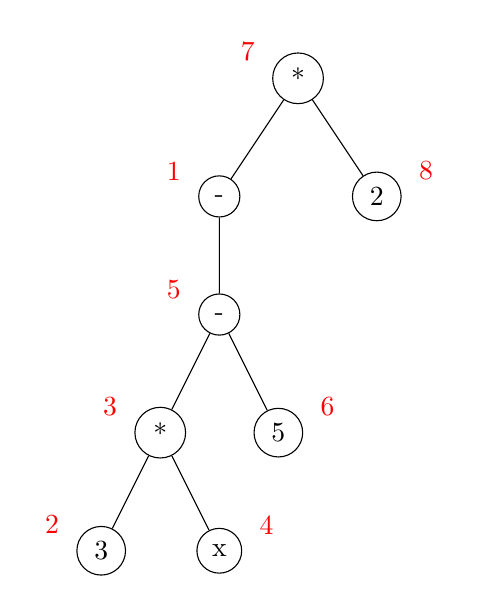
\begin{tikzpicture}[
      level distance=1.5cm,
      level 1/.style={sibling distance=2cm},
      level 2/.style={sibling distance=2cm},
      level 3/.style={sibling distance=1.5cm},
      every node/.style={draw, circle, align=center},
    ]
      \node[label={[label distance=0.1cm, text=red]165:7}] {*}
        child {
          node[label={[label distance=0.1cm, text=red]165:1}] {-}
          child {
            node[label={[label distance=0.1cm, text=red]165:5}] {-}
            child {
              node[label={[label distance=0.1cm, text=red]165:3}] {*}
              child {
                node[label={[label distance=0.1cm, text=red]165:2}] {3}
              }
              child {
                node[label={[label distance=0.1cm, text=red]15:4}] {x}
              }
            }
            child {
              node[label={[label distance=0.1cm, text=red]15:6}] {5}
            }
          }
        }
        child {
          node[label={[label distance=0.1cm, text=red]15:8}] {2}
        };
    \end{tikzpicture}
    \caption{\\Modificeret Inorder Travesal}
  \end{subfigure}
  \hfill
  \begin{subfigure}{0.3\textwidth}
    \centering
    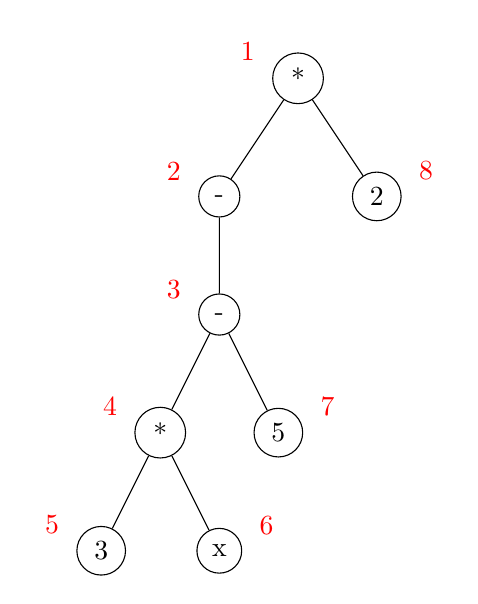
\begin{tikzpicture}[
      level distance=1.5cm,
      level 1/.style={sibling distance=2cm},
      level 2/.style={sibling distance=2cm},
      level 3/.style={sibling distance=1.5cm},
      every node/.style={draw, circle, align=center},
    ]
      \node[label={[label distance=0.1cm, text=red]165:1}] {*}
        child {
          node[label={[label distance=0.1cm, text=red]165:2}] {-}
          child {
            node[label={[label distance=0.1cm, text=red]165:3}] {-}
            child {
              node[label={[label distance=0.1cm, text=red]165:4}] {*}
              child {
                node[label={[label distance=0.1cm, text=red]165:5}] {3}
              }
              child {
                node[label={[label distance=0.1cm, text=red]15:6}] {x}
              }
            }
            child {
              node[label={[label distance=0.1cm, text=red]15:7}] {5}
            }
          }
        }
        child {
          node[label={[label distance=0.1cm, text=red]15:8}] {2}
        };
    \end{tikzpicture}
    \caption{\\Preorder Traversal}
  \end{subfigure}
  \hfill
  \begin{subfigure}{0.3\textwidth}
    \centering
    \begin{tikzpicture}[
      level distance=1.5cm,
      level 1/.style={sibling distance=2cm},
      level 2/.style={sibling distance=2cm},
      level 3/.style={sibling distance=1.5cm},
      every node/.style={draw, circle, align=center},
    ]
      \node[label={[label distance=0.1cm, text=red]165:8}] {*}
        child {
          node[label={[label distance=0.1cm, text=red]165:6}] {-}
          child {
            node[label={[label distance=0.1cm, text=red]165:5}] {-}
            child {
              node[label={[label distance=0.1cm, text=red]165:3}] {*}
              child {
                node[label={[label distance=0.1cm, text=red]165:1}] {3}
              }
              child {
                node[label={[label distance=0.1cm, text=red]15:2}] {x}
              }
            }
            child {
              node[label={[label distance=0.1cm, text=red]15:4}] {5}
            }
          }
        }
        child {
          node[label={[label distance=0.1cm, text=red]15:7}] {2}
        };
    \end{tikzpicture}
    \caption{\\Postorder Traversal}
  \end{subfigure}
  \begin{align*}
      \text{Modificeret Inorder Traversal:} \quad & - (3 \cdot x - 5) \cdot 2 \\
      \text{Preorder Traversal:} \quad &  \cdot - - \cdot 3\, x\, 5\, 2  \\
      \text{Postorder Traversal:} \quad & 3\, x\, \cdot 5\, - -  2\, \cdot
  \end{align*}
  \caption{Træet fra Figur \ref{fig:expression_tree} med forskellige travesal metoder}
  \label{fig:expression_tree_traversal}
\end{figure}


Vi vil i \ref{sec:expression_module} betragte hvordan vi kan implementere et modul som kan repræsentere udtryk ved brug af prefix notation.
Postorder Traversal bliver blandt andet anvendt til at kunne rekursivt simplificere og evaluere udtryk.

Grundet præcedens regler i infix notation, er det nødvendigt at modificere Inorder Traversal, da unære noder altid skal håndteres før dens børn. Desuden vil det også være nødvendigt at implementere regler for at håndtere parenteser, hvis der ønskes et symbolsk udtryk. Den modificeret Inorder Traversal anvendes til at kunne visualisere udtrykket i infix notation.


\subsubsection{Udtryksmodulet}\label{sec:expression_module}
Efter udviklingen af et modul til repræsentation af talmængder er vi nu klar til at udvide programmet med et modul for matematiske udtryk. Vi starter med at definere en polymorf type for udtryk, som beskrevet i Listing \ref{expr_type}. Denne type omfatter flere konstruktører, hver tilknyttet specifikke matematiske operationer vi ønsker at implementere. Desuden introducerer vi konstruktøren \texttt{N} til at repræsentere numeriske værdier ved at anvende talmængder defineret i Listing \ref{number_type}. Til sidst tilføjer vi konstruktøren \texttt{X} for variable. Således lagres matematiske udtryk i en træstruktur, se \ref{sec:expression_as_trees}, eftersom hver konstruktør for en operation indeholder et eller to underudtryk af samme type.


\begin{lstlisting}[
    language={FSharp}, 
    label={expr_type}, 
    caption={Typen for Expr}
    ]
type Expr<'a> = 
    | X of char
    | N of 'a
    | Neg of Expr<'a>
    | Add of Expr<'a> * Expr<'a>
    | Sub of Expr<'a> * Expr<'a>
    | Mul of Expr<'a> * Expr<'a>
    | Div of Expr<'a> * Expr<'a>
\end{lstlisting}

Expr\textless'a\textgreater{}  typen er dermed en polymorfisk type, hvor 'a er typen for den tal mængde hvor vi kan lave brugerdefinerede matematiske operationer. Et exemplar på en Expr\textless Number\textgreater{}  er givet i Listing \ref{lst:expr_example}. Her ses det at når udtrykket $-(3 \cdot x - 5) \cdot 2$ visualiseres er det i prefix notation.

\begin{lstlisting}[style=output, label={lst:expr_example}, caption={$-(3 \cdot x - 5) \cdot 2$ som et udtryks træ. Funktionen tree bliver beskrevet i \ref{sec:expression_generation}.}]
> tree "-(3*x-5)*2";;
val it: Expr<Number> = 
  Mul (Neg (Sub (Mul (N (Int 3), X 'x'), N (Int 5))), N (Int 2))
\end{lstlisting}

Signatur filen indeholder overloadings på de matematiske operationer, så de kan anvendes på udtryk. Samt en funktion \textcolor{red}{eval} til at evaluere et udtryk beskrevet i \ref{sec:eval}. 
\lstinputlisting[
    language=FSharp,
    label={Expression.fsi},
    caption={Signatur filen for Expression modulet}
    ]{../modules/Expression.fsi}



De overloadede matematiske operatorer i Expressions, laver overflade evalueringer samt simplifikationer på deres respektive argumenter. Overfalde evaluering vil sige at de individuelle funktioner kun betragter de to øverste niveauer på de udtryks træer de tager som input, mullige implementeringer af addition og multiplikation er givet i Listing \ref{lst:mul_expr}. Lignende funktioner er implementeret for de andre operationer.

\begin{lstlisting}[
  language={FSharp}, 
  label={lst:mul_expr}, 
  caption={Addition og multiplikation af to udtryk}
  ]
// mul: Expr<Number> -> Expr<Number> -> Expr<Number>
let rec mul e1 e2:Expr<Number> =
  match e1, e2 with
  |N a, N b                       -> N (a * b)
  |N a, b | b, N a when isOne a   -> b
  |N a, _ | _, N a when isZero a  -> N zero
  |Div(a, b), c | c, Div(a, b)    -> Div (mul a c, b)
  |Div (a, b), Div (c, d)         -> Div ((mul a c), (mul b d))
  |Neg a, Neg b                   -> mul a b
  | _, _                          -> Mul(e1, e2)

// add: Expr<Number> -> Expr<Number> -> Expr<Number>
let rec add e1 e2:Expr<Number>  =
  match e1, e2 with
  | N a, N b                            -> N (a + b)
  | N a, b | b, N a when isZero a       -> b
  | a, b when a = b                     -> Mul (N two, b)
  | Neg a, Neg b                        -> neg (add a b) 
  | Neg a, b | b, Neg a                 -> Sub (b, a)
  | Mul(a, X b), Mul(c, X d) 
  | Mul(X b, a), Mul(c, X d)
  | Mul(a, X b), Mul(X d, c) 
  | Mul(X b, a), Mul(X d, c) when b = d -> Mul(add a c, X b)
  | _, _                                -> Add(e1, e2)

\end{lstlisting}

\subsection{Evaluering af udtryk}\label{sec:eval}
Vi vil nu betragte hvordan vi kan evaluere et udtryk, ved hjælp af et miljø som indeholder værdier for variable som er indeholdt i udtrykket. Evalueringen af udtryk skal kunne opfylde følgende homomorfiske egenskaber \ref{prop:eval_homomorphism}. Egenskaben vil blive testet i sektion \ref{sec:PBT_eval_homomorphism}.
\vspace{0.5cm}
\begin{egenskab}[Homomorfisme af evaluering]\label{prop:eval_homomorphism}
Lad $\oplus \in \{+, -, \times, /\}$ sættet af binære operationer, $e1$ og $e2$ være udtryk, så gælder følgende:
\begin{align*}
    \text{eval}(e1 \oplus e2) = \text{eval}(e1) \oplus \text{eval}(e2)
\end{align*}
Derudover skal det om negation også gælde at:
\begin{align*}
    \text{eval}(-e) = -\text{eval}(e)
\end{align*}
\end{egenskab}


Funktionen \textcolor{red}{eval} i Listing \ref{lst:eval_expr} tager et udtryk og et miljø som input og evaluere udtrykket til en numerisk værdi. Funktionen kører en Postorder Traversal på udtrykket og evaluerer dermed udtrykket nedefra og op, ved at foretage matematiske operationer defineret i Number modulet. 

\begin{lstlisting}[
  language={FSharp}, 
  label={lst:eval_expr}, 
  caption={Evaluering af et udtryk}
  ]
// eval: Expr<Number> -> Map<char, Number> -> Number
let rec eval (e:Expr<Number>) (env) =
  match e with
  | X x -> Map.find x env
  | N n -> n
  | Neg a -> - eval a env
  | Add (a, b) -> eval a env + eval b env
  | Sub (a, b) -> eval a env - eval b env
  | Mul (a, b) -> eval a env * eval b env
  | Div (a, b) -> eval a env / eval b env
\end{lstlisting}

\subsection{Konventering mellem udtryks notation}\label{sec:expression_generation}
Det er ønkes at kunne konvertere udtryk frem og tilbage mellem prefix notation, repræsenteret af Expression-typen, og den standard infix notation. Dette ønske skyldes, at infix notation er lettere for os at læse og skrive. Derfor er det essentielt, at de to konverteringsfunktioner fungerer som hinandens inverser. Dette krav er yderligere uddybet i egenskab \ref{egenskab:infix_prefix}. Egenskaben bliver test i sektion \ref{sec:PBT_infix_prefix}.

\vspace{0.5cm}
\begin{egenskab}[Invers morphism\footcitetitle{Inverse_function} mellem infix og prefix]\label{egenskab:infix_prefix}
    Lad $Q^n$ være mængden af rationelle infix udtryk repræsenteret som en string, med $n$ variable, så defineres følgende:
    \begin{align*}
      \text{tree}&: Q^n \to \text{Expr} \\
      \text{tree}^{-1}&: \text{Expr} \to  Q^n  
    \end{align*}
    Dermed gælder følgende egenskaber
    \begin{align*}
      \text{tree}^{-1} \circ \text{tree} &= id_{Q^n} \\
      \text{tree} \circ \text{tree}^{-1} &= id_{\text{Expr}}
    \end{align*}
    Hvor $id_{x}$ er identitetsfunktionen på mængden $x$.
\end{egenskab}

Vi begynder med at betragte den inverse funktion, som konverterer fra en expression til infix notation. Funktionen \textcolor{red}{etf} se Listing \ref{lst:expression_to_infix} fortager denne konventering ved at lave en modificeret Inorder Traversal på udtrykket, som beskrevet i \ref{sec:expression_as_trees}. Den modificeret del er at håndtere parenteser samt håndtere negation som var det en binær node i træet hvor det venstre barn er et tomt udtryk.

\begin{lstlisting}[
  language={FSharp}, 
  label={lst:expression_to_infix}, 
  caption={konventering fra expression til infix notation}
  ]
// parenthesis: bool -> string -> string
let parenthesis b f = if b then "(" + f + ")" else f

// etf: Expr<Number> -> bool -> string
let rec etf e p =
    match e with
    | N a when not <| isInt a -> parenthesis p <| toString a
    | N a   -> toString a
    | X a   -> string a
    | Neg a -> parenthesis p <| "-" + etf a (not p) 
    | Add(a, b) -> parenthesis p <| etf a false + "+" + etf b false
    | Sub(a, b) -> parenthesis p <| etf a false + "-" + etf b true
    | Mul(a, b) -> parenthesis p <| etf a true  + "*" + etf b true
    | Div(a, b) -> parenthesis p <| etf a true  + "/" + etf b true


// infixExpression: Expr<Number> -> string
let infixExpression e = etf e false
\end{lstlisting}

Funktionen \textcolor{red}{\texttt{tree}}, som foretager konverteringen fra infix notation til et udtrykstræ, er baseret på algoritmen beskrevet i \cite{convert_expression}\footcitetitle{convert_expression}. Først konverteres en udtryksstreng til en liste af tokens. Disse tokens beskriver, om en karakter i udtrykket er en operand, en operator, eller en konstant, hvor en operator også indeholder information om præcedens og associativitet\footcitetitle{precedens_associativity}. Typen for disse tokens kan ses i Listing \ref{lst:infix_to_expression_types}. Herefter anvendes to stacks: én for operatorer og én for udtryk. Der anvendes en række regler, som beskrevet i \cite{convert_expression}, for hvornår der skal udføres pop og push på disse to stacks. Det skal bemærkes, at når en operator pushes til udtryksstacken, da navnet på operatorkonstruktøren på udtrykket står skrevet fra venstre mod højre, vil udtryksstacken være i prefix notation og ikke postfix notation som beskrevet i kilden. Funktionen \textcolor{red}{\texttt{tree}} er at finde i Appendiks \ref{sec:treeGenerator.fs}.

\begin{lstlisting}[
  language={FSharp}, 
  label={lst:infix_to_expression_types}, 
  caption={Konvertering fra infix til udtrykstræ}
]
type Associative = | Left | Right
type Precedence = int
type Operator = char * Precedence * Associative
type Token =
    | Operand of char
    | Operator of Operator
    | Constant of int
type OperatorList = Operator list
\end{lstlisting}




\subsection{Simplifikation af udtryk} \label{sec:simplification_expression}
Vi skal nu betragte en sytematisk metode til at kunne simplificere matematiske udtryk, ved hjælp af simple algebraiske regler. Dette er en nødvendig at kunne for at bruge udtrykkene i en matematisk sammenhæng, da det vil kunne medføre både en reduktion i kompleksitet og en forbedring i læsbarhed når udtrykene visualiseres. Før vi betragter metoden, kan vi opskrive en egenskab som simplification skal overholde. Egenskaben vil blive testet i sektion \ref{sec:PBT_simplification}, det er en nødvendighed at evaluere udtrykket før og efter simplifikationen da det er en kompleks opgave at skulle sammenligne om to udtryk er ækvivalente.
\vspace{0.5cm}
\begin{egenskab}[Simplifikation af udtryk]\label{egenskab:simplification}
Lad $e$ være et udtryk, så gælder følgende:
\begin{align*}
  \text{eval}(e) = \text{eval}(\text{simplifyExpr}(e))
\end{align*}
\end{egenskab}

Vi begynder med at betragte funktionen \textcolor{red}{\texttt{simplifyExpr}} i Listing \ref{lst:simplify_expr}, som simplificerer et udtryk ved at foretage en Postorder Traversal på udtrykket. På den måde sikre sig at når en node i udtrykstræet bliver simplificeret, vil dens børn allerede være simplificeret. 

\begin{lstlisting}[
  language={FSharp}, 
  label={lst:simplify_expr}, 
  caption={Simplifikation af et udtryk}
  ]
  //simplifyOperation: Expr<Number> -> Expr<Number> -> (Expr<Number> -> Expr<Number> -> Expr<Number>) -> Expr<Number>
  let rec simplifyOperation e1 e2 f = 
  match f e1 e2 with
  | Neg a -> 
    commutativeMulDiv.applyCommutative (Neg a) |> commutativeAddSub.applyCommutative
  | Add(a, b) when isAdd f -> commutativeAddSub.applyCommutative (Add(a, b))
  | Sub(a, b) when isSub f -> commutativeAddSub.applyCommutative (Sub(a, b))
  | Mul(a, b) when isMul f -> commutativeMulDiv.applyCommutative (Mul(a, b))
  | Div(a, b) when isDiv f -> commutativeMulDiv.applyCommutative (Div(a, b))
  | Add(a, b) -> simplifyOperation a b (+)
  | Sub(a, b) -> simplifyOperation a b (-)
  | Mul(a, b) -> simplifyOperation a b (*)
  | Div(a, b) -> simplifyOperation a b (/)
  | a -> a


//simplifyExpr: Expr<Number> -> Expr<Number>
let rec simplifyExpr e =
  match e with
  | N a when Number.isNegative a -> Neg (N (Number.absNumber a))
  | N (Rational(R(a, b))) -> 
    simplifyOperation (simplifyExpr (N (Int a))) (simplifyExpr (N (Int b))) (/)
  | Neg a     -> - (simplifyExpr a)
  | Add(a, b) -> simplifyOperation (simplifyExpr a) (simplifyExpr b) (+)
  | Sub(a, b) -> simplifyOperation (simplifyExpr a) (simplifyExpr b) (-)
  | Mul(a, b) -> simplifyOperation (simplifyExpr a) (simplifyExpr b) (*)
  | Div(a, b) -> simplifyOperation (simplifyExpr a) (simplifyExpr b) (/)
  | _ -> e 
\end{lstlisting}

Det er \textcolor{red}{simplifyOperation}, som foretager selve simplificeringen af et givet udtryk. Funktionen tager som input to udtryk samt den binære operation, der skal anvendes på disse. Funktionen anvendes på udtrykkene, hvorefter overfladisk simplifikation, som blev beskrevet i \ref{sec:expression_module}, udføres. Hvis overfladisk simplifikation resulterer i en ændring af den anvendte operation, kalder funktionen sig selv rekursivt med de to udtryk og den nye operation. Hvis overfladisk simplifikation ikke resulterer i ændringer i operationen, vil funktionen foretage en dybere simplifikation af de to udtryk. Denne dybere simplifikation udføres af funktionerne \textcolor{red}{applyCommutative} fra filerne \textit{CommutativeAddSub.fs} og \textit{CommutativeMulDiv.fs}, som findes i Appendiks \ref{sec:commutativeAddSub.fs} og \ref{sec:commutativeMulDiv.fs}. Disse funktioner arbejder efter samme princip, hvor de starter med at flade udtrykstræerne ud ifølge de kommutative regler for henholdsvis addition og multiplikation. Derefter sorterer de udtrykstræet, hvilket muliggør at foretage overfladisk når ved at gendanne træet. For multiplikation anvendes samme metode i nævneren for division, og der undersøges, om der er fælles udtryk i det udfladede træ, som fremtræder i nævneren af en division og i det udfladede træ, der indeholder divisionen. Et eksempel på anvendelse af den kommutative multiplikationssimplifikation på et udtryk er givet i Figur \ref{fig:expression-trees}, som viser det visuelle input og det resulterende svar fra funktionen, samt Figur \ref{fig:trees}, der viser det udfladede træ og sorteringen af det fladede træ.


\begin{figure}[H]
  \centering
  \begin{subfigure}[b]{0.5\textwidth}
    \centering
    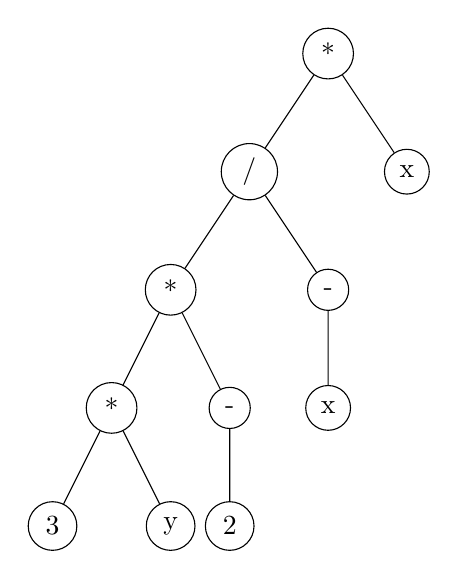
\begin{tikzpicture}[
      level distance=1.5cm,
      level 1/.style={sibling distance=2cm},
      level 2/.style={sibling distance=2cm},
      level 3/.style={sibling distance=1.5cm},
      every node/.style={draw, circle, align=center},]
      \node {*}
        child { node {/}
          child { node {*}
            child { node {*}
              child { node {3}
              }
              child { node {y}
              }
            }
            child { node {-}
              child { node {2}
              }
            }
          }
          child { node {-}
            child { node {x}
            }
          }
        }
        child { node {x}
        };
    \end{tikzpicture}
    \caption{Udtrykket $(3 \cdot y \cdot (-2)/-x) \cdot x$ som et træ}
    \label{fig:original-tree}
  \end{subfigure}
  \hfill
  \begin{subfigure}[b]{0.4\textwidth}
    \centering
    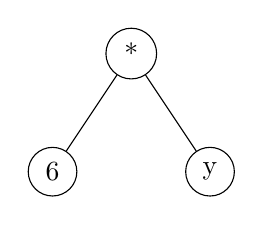
\begin{tikzpicture}[
      level distance=1.5cm,
      level 1/.style={sibling distance=2cm},
      every node/.style={draw, circle, align=center},]
      \node {*}
        child { node {6} }
        child { node {y} };
    \end{tikzpicture}
    \caption{Det resuterende simplificerede efter at have anvendt CommutativeMulDiv.\textcolor{red}{applyCommutative} på udtrykket i Figur \ref{fig:original-tree}}
    \label{fig:simplified-tree}
  \end{subfigure}
  \caption{Før og efter simplifikation af et udtryk ved brug af CommutativeMulDiv.\textcolor{red}{applyCommutative}}
  \label{fig:expression-trees}
\end{figure}


% Flattened Tree
\begin{figure}[H]
  \centering
  \begin{subfigure}[b]{0.45\textwidth}
    \centering
    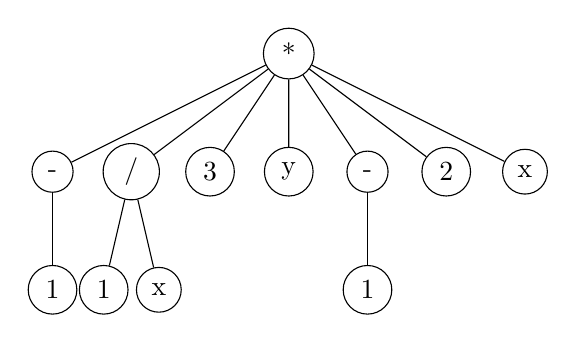
\begin{tikzpicture}[level distance=1.5cm,
      level 1/.style={sibling distance=1cm},
      level 2/.style={sibling distance=0.7cm},
      level 3/.style={sibling distance=1.5cm},
      every node/.style={draw, circle, align=center},]89
      \node {*}
        child{ node {-} 
          child { node {1}}}
        child { node {/}
          child { node {1}
          }
          child { node {x}}
        }
        child { node {3}
        }
        child { node {y}
        }
        child { node {-}
          child { node {1}
          }
        }
        child { node {2}
        }
        child { node {x}
        };
    \end{tikzpicture}
    \caption{Det udfladede træ}
    \label{fig:sub1}
  \end{subfigure}
  \hfill
  \begin{subfigure}[b]{0.45\textwidth}
    \centering
    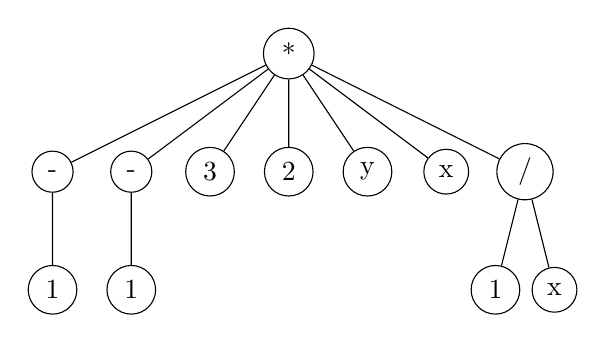
\begin{tikzpicture}[level distance=1.5cm,
      level 1/.style={sibling distance=1cm},
      level 2/.style={sibling distance=0.75cm},
      level 3/.style={sibling distance=1cm},
      every node/.style={draw, circle, align=center},]
      \node {*}
        child { node {-}
          child { node {1} }
        }
        child { node {-}
          child { node {1} }
        }
        child { node {3} }
        child { node {2} }
        child { node {y} }
        child { node {x} }
        child { node {/}
          child { node {1} }
          child { node {x} }
        };
    \end{tikzpicture}
    \caption{Det sorterede træ fra venstre mod højre}
    \label{fig:sub2}
  \end{subfigure}
  \caption{Det udfladede og sorterede af udtrykket $(3 \cdot y \cdot (-2)/-x) \cdot x$ i processen af kommutativ simplifikation}
  \label{fig:trees}
\end{figure}

Generelt, når det gælder simplificering af udtryk, skal man være opmærksom på ikke at ende i et uendeligt loop. Derfor er det vigtigt ikke at definere nogle overfladiske simplificeringer, som er hinandens inverse funktioner. Desuden forsøger funktionerne i dette program altid at skubbe negation af udtryk så langt ud som muligt i håb om, at de kan ophæve hinanden. Dette illustreres blandt andet i figur \ref{fig:trees}, hvor ved udfladning af træet, hvis et af de kommutative udtryk for multiplikation er negativt, fjernes negationen, og der tilføjes i stedet en negation af tallet 1, som ved sortering skubbes til venstre.


\subsection{Differentiering af udtryk}
Vi kan nu betragte den første implementering, der benytter vores udtryksmodul, som samtidig vil understrege vigtigheden af at kunne simplificere udtryk. Vi begynder igen med at opskrive nogle algebraiske linearitetsegenskaber, som differentieringen skal overholde. Disse egenskaber vil blive testet i sektion \ref{sec:PBT_differentiation}.
\vspace{0.5cm}
\begin{egenskab}[Linearitetsbetingelserne\footcitetitle{diff}]\label{egenskab:differentiation}
  Lad $f$ og $g$ være udtryk, og $a$ være tal fra talmodulet, så gælder følgende:
  \begin{enumerate}
    \item \textbf{Skaleringsreglen} \\
    \(\frac{d}{dx}(af) = a\frac{df}{dx}\)
    \item \textbf{Sumreglen} \\
    \(\frac{d}{dx}(f+g) = \frac{df}{dx} + \frac{dg}{dx}\)
    \item \textbf{Subtraktionsreglen} \\
    \(\frac{d}{dx}(f-g) = \frac{df}{dx} - \frac{dg}{dx}\)
    \item \textbf{Produktreglen} \\
    \(\frac{d}{dx}(fg) = \frac{df}{dx}g + f\frac{dg}{dx}\)
    \item \textbf{Kvotientreglen} \\
    \(\frac{d}{dx}\left(\frac{f}{g}\right) = \frac{\frac{df}{dx}g - f\frac{dg}{dx}}{g^2}\)
  \end{enumerate}
\end{egenskab}

Funktionen for differentiering \textcolor{red}{diff} i Listing \ref{lst:diff_expr}, som tager et udtryk og en variabel som input og differentierer udtrykket med hensyn til variablen. Dette er en af de store fordele ved at anvende et funktionelt programmeringssprog, da det ses, hvordan fire af reglerne fra egenskab \ref{egenskab:differentiation} er implementeret direkte, som de er beskrevet.

\begin{lstlisting}[
  language={FSharp}, 
  label={lst:diff_expr}, 
  caption={Differentiering af et udtryk}
  ]
// diff: Expr<Number> -> char -> Expr<Number>
let rec diff e dx = 
    match e with
    | X f when f = dx -> N (Int 1)
    | X _ -> N (Int 0)
    | N _ -> N (Int 0)
    | Neg f -> diff (Mul (N (Int -1), f)) dx
    | Add(f, g) -> Add(diff f dx, diff g dx)
    | Sub(f, g) -> Sub(diff f dx, diff g dx)
    | Mul(f, g) -> Add(Mul(diff f dx, g), Mul(f, diff g dx))
    | Div(f, g) -> Div(Sub(Mul(diff f dx, g), Mul(f, diff g dx)), Mul(g, g))
\end{lstlisting}


\subsection{Multivariable polynomier af første grad}
Da vi senere i projektet skal betragte matricer, vil vi i den forbindelse også lave en løsning af lineære ligningssystemer i sektion \ref{sec:lin_eq}. Det kræver derfor, at vi kan isolere variable i et multivariabelt polynomium af første grad. Vi betragter derfor nu to simple funktioner til at udføre denne isolation, se Listing \ref{lst:isolate}. Funktionen \textcolor{red}{isolateX} undersøger først, om den variabel, som skal isoleres, befinder sig på højre eller venstre side, derefter kaldes funktionen \textcolor{red}{expressionOnX}, som fungerer ved at evaluere til en funktion, der giver den omvendte operation af den operation, som variablen er involveret i. Dertil anvendes den omvendte funktion på begge sider af ligningen, hvor hvis variablen er isoleret, gives et udtrykspar, hvor det første udtryk er den isolerede variabel. Hvis variablen ikke er isoleret, kaldes funktionen rekursivt med de nye højre og venstre sider.

\begin{lstlisting}[
  language={FSharp}, 
  label={lst:isolate}, 
  caption={Isolering af variable i et udtryk}
  ]
// expressionOnX: Expr<'a> -> Expr<'a> -> (Expr<'a> -> Expr<'a>)
let rec expressionOnX hs x =
  match hs with
  | N _ | X _ -> fun e -> e
  | Neg(a) when a = x -> fun e -> Neg e
  | Sub(a, b) when a = x -> fun e -> Add(e, b)
  | Div(a, b) when a = x -> fun e -> Mul(e, b)
  | Div(_, a) when a = x -> fun e -> Mul(e, a)
  | Mul(a, b) | Mul(b, a) when a = x -> fun e -> Div(e, b)
  | Add(a, b) | Add(b, a) | Sub(b, a) when a = x -> fun e -> Sub(e, b)
  | Add(a, b) | Sub(a, b) | Mul(a, b) | Div(a, b) -> fun e -> expressionOnX a x e |> expressionOnX b x 
  | Neg(a) -> fun e -> expressionOnX a x e

// isolateX: Expr<Number> -> Expr<Number> -> Expr<Number> -> Expr<Number> * Expr<Number> 
let rec isolateX lhs rhs x =
  let operation = 
      if containsX lhs x 
          then expressionOnX lhs x
      elif containsX rhs x 
          then expressionOnX rhs x
      else 
          failwith "Variable not found in either side of the equation"
  match operation lhs |> simplifyExpr, operation rhs |> simplifyExpr with
  | a, b | b, a when a = x -> (a, b)
  | a, b -> isolateX a b x
\end{lstlisting}

Da funktionen kun betragter operationen på den variable, der ønskes isoleret, eksisterer der mange tilfælde, hvor funktionen ikke vil kunne isolere variablen. Men den fungerer til at løse ligninger af formen \(a_1x_1 + a_2x_2 + \ldots + a_nx_n = b\), hvilket er tilstrækkeligt for vores formål.

\newchapter
\section{Vektorer og Matricer}
Vi vil nu betragte opbyggelsen af et modul for vektorer og matricer. Eftersom en vektor også kan opfattes som en matrix, vil vi i det følgende, når begge dele omtales, udelukkende referere til matricer. For systematik at kunne håndtere matricer, starter vi med at definere en type for lagringsordning Listing \ref{Order}.

\begin{lstlisting}[
    language={FSharp}, 
    label={Order}, 
    caption={Typen for order}
    ]
type Order = | R | C
\end{lstlisting}

Typen Order, anvendes til at angive, om en matrix er i rækkefølge (row-major) eller kolonnefølge (column-major)\footcitetitle{major_order}. En vektor, der er lagret i rækkefølge, kan betragtes som den transponeret kolonnefølge vektor. Vi kan derfor nu definere en type for matricer, ved hjælp af en type for vektore i Listing \ref{matrix}.

\begin{lstlisting}[
    language={FSharp}, 
    label={matrix}, 
    caption={Typen for Matricer}
    ]
type Vector = V of list<Number> * Order
type Matrix = M of list<Vector> * Order
\end{lstlisting}

Derudover er det en fordel at kunne kende dimissionen af en matrix. Derfor er der også defineret en type for dimissionen se Listing \ref{dim}.

\begin{lstlisting}[
    language={FSharp}, 
    label={dim}, 
    caption={Typen for dimissionen}
    ]
// Rows x Cols
type Dimension = D of int * int
\end{lstlisting}


\subsection{Matrix operationer}
Der vil i denne sektion beskrives en række funktioner som er nødvendige før vi kan betragte nogle funktion for anvendelse af matricer. Da modulet indeholder mange hjælpe funktioner, vil der fokuseres på de funktioner med matematisk relevans.

Det muligt at definere en funktion til at finde dimissionen af en matrix se Listing \ref{dim_func}. Funktionen laver et kald til \textcolor{red}{matrixValidMajor} som genere en fejl hvis ikke alle vektorer og matrien har samme lagringsordning. \textcolor{red}{matrixVectorLength} finder længden på vektor listen en i matricen.

\begin{lstlisting}[
    language={FSharp}, 
    label={dim_func}, 
    caption={Funktion til at finde dimissionen af en matrix}
    ]
    // dimMatrix : Matrix -> Dimension
let dimMatrix (M(vl, o)) =
    if vl = [] then D (0, 0)
    else
    let _ = matrixValidMajor (M(vl, o))
    let d1 = List.length vl
    let d2 = matrixVectorLength (M(vl, o))
    match o with
    | R -> D (d1, d2)
    | C -> D (d2, d1)
\end{lstlisting}

Hvis en matrix er gemt som rækkefølge, vil antallet af rækker være længden af en vektor og antallet af kolonner være længden af vektor listen, og omvendt for kolonnefølge.

\subsection{Matematiske operationer}
I denne sektion bør det bemærkes, at flere listings ikke inkluderer fejlhåndtering; dette er udeladt for at forbedre læsbarheden. De funktioner, der anvendes i det implementerede modul, har passende fejltjek, herunder dimensionstjek på matricerne. Den fulde implementering med fejlhåndtering kan findes i appendiks \ref{sec:matrix.fs}.

Før vi implementere funktioner til at udføre de ønskede matematiske operationer, vil vi først definere nogle egenskaber matricerne skal opfylde i egenskab \ref{vector_space_axioms}.
\vspace{0.5cm}
\begin{egenskab}[Vektor Aksiomer]\label{vector_space_axioms}
    Lad $c, d \in \mathbb{F}$ og $v_i \in \mathbb{F}^n$ for $i = 1 \dots m$ så gælder:\footcitetitle[Theorem 7.2 s. 155]{mat1a}
    \begin{enumerate}
        \item $(v_1 + \dots + v_{m-1}) + v_m = v_1 + (v_2 + \dots + v_m)$
        \item $c \cdot \left(d \cdot \begin{bmatrix}
            | &        & | \\
            v_{1} & \cdots & v_{m} \\
            | &        & | \\
        \end{bmatrix}\right) = (c \cdot d) \cdot \begin{bmatrix}
            | &        & | \\
            v_{1} & \cdots & v_{m} \\
            | &        & | \\
        \end{bmatrix}$
        
        \item $c \cdot (v_1 + \dots +v_m) = c \cdot v_1 + \dots +c \cdot v_m$
    \end{enumerate}
\end{egenskab}


\subsubsection{Skalering af en matrix}
Vi begynder med at betragte en funktion til at skalere en matrix se Listing \ref{scale_matrix}. 

\begin{lstlisting}[
    language={FSharp}, 
    label={scale_matrix}, 
    caption={Funktion til at skalere en matrix}
    ]
// scalarVector : Number -> Vector -> Vector
let scalarVector (n:Number) (V (nl, o)) = 
    V ((List.map (fun x -> x * n) nl), o)

// scalarMatrix : Matrix -> Number -> Matrix
let scalarMatrix (M (vl, o)) n = 
    M ((List.map (fun x -> scalarVector n x) vl), o)
\end{lstlisting}

Det at skalere en matrice er svare til at skalere hvert element i matricen. Derfor ved at have en funktion \textcolor{red}{scalarVector}, der skalere hvert element i en givet vektor bliver \textcolor{red}{scalarMatrix} at skalere hver vektor i en givet matrice. List.\textcolor{red}{map} svare til at lave en list comprehension i Python\footcitetitle{list_comprehension}.


\subsubsection{Addition af matricer}
\begin{lstlisting}[
    language={FSharp}, 
    label={add_matrix}, 
    caption={Funktion til at addere matricer og substraktion af vektorer}
    ]
// addVector : Vector -> Vector -> Vector
let addVector (V (v1, o1)) (V (v2, _)) =
    V ((List.map2 (+) v1 v2), o1)

// addMatrix : Matrix -> Matrix -> Matrix
let addMatrix (M(vl1, o)) (M(vl2, _)) =
    M (List.map2 addVector vl1 vl2, o)

// subVector : Vector -> Vector -> Vector
let subVector x y =
    scalarVector (-one) y |> addVector x
    
// sumRows : Matrix -> Matrix
let rec sumRows m = 
    if not <| corectOrderCheck m C 
        then sumRows <| correctOrder m C
    else
        let zeroVector = vectorOf zero <| matrixVectorLength m
        let (M(vl, _)) = m
        matrix [List.fold (addVector) zeroVector vl]
\end{lstlisting}

Addition af vektorer reduceres til at udføre additionen elementvis, som vist i Listing \ref{add_matrix}, ved brug af List-funktionen \textcolor{red}{map2}. Vi kan bruge \textcolor{red}{addVector} til at definere matrix addition og subtraktion af vektorer. Vektor addition bruges også til at summere rækkerne i en matrix (\textcolor{red}{sumRows}), hvilket vil blive anvendt i implementeringen af matrix produkt i næste sektion og Gram-Schmidt-processen i sektion \ref{sec:gram_schmidt}. Funktionen bliver yderligere beskrevet i definition \ref{sumRows}.

\vspace{0.5cm}
\begin{definition}[Summering af rækker i en matrix] \label{sumRows}
Lad $A$ være en matrix med $m$ rækker og $n$ søjler, hvor
\[
A = \begin{bmatrix}
a_{11} & a_{12} & \cdots & a_{1n} \\
a_{21} & a_{22} & \cdots & a_{2n} \\
\vdots & \vdots & \ddots & \vdots \\
a_{m1} & a_{m2} & \cdots & a_{mn}
\end{bmatrix}
\]

Så gælder om \textcolor{red}{sumRows} at

\[
\textit{\textcolor{red}{sumRows}}(A) =
v = \begin{bmatrix}
\sum_{j=1}^{n} a_{1j} \\
\sum_{j=1}^{n} a_{2j} \\
\vdots \\
\sum_{j=1}^{n} a_{mj}
\end{bmatrix}
\]

Dermed er $v_i = \sum_{j=1}^{n} a_{ij}$ for $i = 1, 2, \ldots, m$.
\end{definition}

\subsubsection{Matrix produkt}


\begin{definition}[Matrix-Vektor Produkt] \label{def:matrix_vector_pro}
    Lad $A$ være en matrix med $m$ rækker og $n$ søjler, hvor
    \[
    A = \begin{bmatrix}
    a_{11} & a_{12} & \cdots & a_{1n} \\
    a_{21} & a_{22} & \cdots & a_{2n} \\
    \vdots & \vdots & \ddots & \vdots \\
    a_{m1} & a_{m2} & \cdots & a_{mn}
    \end{bmatrix}
    \]
    og $\mathbf{v} = (v_1, v_2, \ldots, v_n)^T$ være en vektor med $n$ elementer. Så er matrix-vektor $Av$ produktet defineret som
    \[
\begin{bmatrix}
    a_{11} & a_{12} & \cdots & a_{1n} \\
    a_{21} & a_{22} & \cdots & a_{2n} \\
    \vdots & \vdots & \ddots & \vdots \\
    a_{m1} & a_{m2} & \cdots & a_{mn}
\end{bmatrix}
\begin{bmatrix}
    v_{1} \\
    v_{2} \\
    \vdots \\
    v_{n}
\end{bmatrix}
=
\begin{bmatrix}
    a_{11}v_{1} + a_{12}v_{2} + \cdots + a_{1n}v_{n} \\
    a_{21}v_{1} + a_{22}v_{2} + \cdots + a_{2n}v_{n} \\
    \vdots \\
    a_{m1}v_{1} + a_{m2}v_{2} + \cdots + a_{mn}v_{n}
\end{bmatrix}
= \begin{bmatrix}
    \sum_{j=1}^{n} a_{1j}v_{j} \\
    \sum_{j=1}^{n} a_{2j}v_{j} \\
    \vdots \\
    \sum_{j=1}^{n} a_{mj}v_{j}
\end{bmatrix}
\]
\end{definition}

\begin{theorem}[Matrix-Vektor Produkt] \label{matrix_vector_pro}
    Lad $A$ være en matrix med $m$ rækker og $n$ søjler, og lad $\mathbf{v}$ være en vektor med $n$ elementer. Så gælder der
    \[ Av = \textit{\textcolor{red}{sumRows}}
    \begin{bmatrix}
        | & | &        & | \\
        a_{1}v_{1} & a_{2}v_{2} & \cdots & a_{n}v_{n} \\
        | & | &        & | \\
    \end{bmatrix}
    \]
\end{theorem}
\begin{proof}
    Lad $B$ være resultatet af at skalere søjlerne i matrix $A$ med de tilsvarende elementer i vektoren $\mathbf{v}$. Vi har
    \begin{alignat*}{2}
    B &= \begin{bmatrix}
        | & | &        & | \\
        a_{1}v_{1} & a_{2}v_{2} & \cdots & a_{n}v_{n} \\
        | & | &        & | \\
    \end{bmatrix} \\
    &= \begin{bmatrix}
        a_{11}v_{1} & a_{12}v_{2} & \cdots & a_{1n}v_{n} \\
        a_{21}v_{1} & a_{22}v_{2} & \cdots & a_{2n}v_{n} \\
        \vdots & \vdots & \ddots & \vdots \\
        a_{m1}v_{1} & a_{m2}v_{2} & \cdots & a_{mn}v_{n}
    \end{bmatrix}
    \end{alignat*}
    Ved brug af definition \ref{sumRows} for \textit{\textcolor{red}{sumRows}} og definition \ref{def:matrix_vector_pro} ses det at 
    \begin{alignat*}{2}
    \text{{\color{red}\textit{sumRows}}}(B) &= \begin{bmatrix}
        \sum_{j=1}^{n} a_{1j}v_{j} \\
        \sum_{j=1}^{n} a_{2j}v_{j} \\
        \vdots \\
        \sum_{j=1}^{n} a_{mj}v_{j}
    \end{bmatrix} = A\mathbf{v}
    \end{alignat*}
\end{proof}
Vi kan dermed anvende sætning \ref{matrix_vector_pro} til at definere en funktion \textcolor{red}{matrixVectorProduct} til matrix-vektor produkt se Listing \ref{vecPro}. Denne funktion skalerer først søjlerne i matricen med de tilsvarende elementer i vektoren og summer derefter rækkerne i matricen.
\begin{lstlisting}[
    language={FSharp}, 
    label={vecPro}, 
    caption={Funktion til matrix-vektor produkt}
    ]
// matrixVectorProduct : Matrix -> Vector -> Matrix
let rec matrixVectorProduct (M(vl, _)) (V(nl, _)) =
    M (List.map2 (fun mc n -> scalarVector n mc) vl nl, C) 
    |> sumRows
\end{lstlisting}

\begin{definition}[Matrix produkt]\label{def:matrix_matrix_pro}
    Lad $A \in \mathbb{F}^{m \times n}$ og $B \in \mathbb{F}^{n \times \ell}$. Lad søjlerne i $B$ er være givet ved $b_1, \ldots, b_\ell \in \mathbb{F}^n$, dermed\footcitetitle[Definition 7.12
 s. 162]{mat1a}
    \[
        B = \begin{bmatrix}
    | &  & | \\
    b_1 & \cdots & b_\ell \\
    | &  & | \\
\end{bmatrix}.
\]
Så defineres matrixproduktet som
\[
    A \cdot B = \begin{bmatrix}
        | &  & | \\
        A \cdot b_1 & \cdots & A \cdot b_\ell \\
        | &  & | \\
    \end{bmatrix}.
    \]
\end{definition}
Ud fra definition \ref{def:matrix_matrix_pro} ses det, at funktionen \textcolor{red}{matrixProduct} i Listing \ref{pro_matrix} til at tage produktet af to matricer, ved at udfører matrix-vektor produkt på hver søjle i matricen. Da \textcolor{red}{matrixVectorProduct} evaluere til en matrix, skal der bruges en funktion til at konvertere matricen til en vektor, hvilket \textcolor{red}{matrixToVector} gør.
\begin{lstlisting}[
    language={FSharp}, 
    label={pro_matrix}, 
    caption={Funktion til at tage produktet af to matricer}
    ]
// matrixProduct : Matrix -> Matrix -> Matrix
let rec matrixProduct a (M(vlb, _)) =
    let product = List.map (
        fun bv -> matrixVectorProduct a bv |> matrixToVector ) vlb
    M(product, C)
\end{lstlisting}
        
\subsubsection{Projektion af en vektor}

\begin{definition}[Projektion af en vektor]\label{def:proj}
Projektionen af en vektor på en linje defineres i som følgende, hvor $Y = \text{span}\{y\}$\footcitetitle[s. 40]{mat1b}.
\begin{align}
    \text{proj}_Y : V \rightarrow V, \quad \text{proj}_Y(x) = \frac{\langle x, y \rangle}{\langle y, y \rangle} y
\end{align}
hvor det standard indre produkt er defineret som:
\begin{align}
    \langle x, y \rangle = y^* x = \sum_{k=1}^{n} x_k \overline{y}_k
\end{align}
\end{definition}
    

For at kunne projektere en vektor, som defineret i destination \ref{def:proj} skal vi først kunne konjugere en vektor. Funktionen \textcolor{red}{conjugateVector} konjugerer elementerne i en vektor. Derudover defineres en funktion til at multiplicere to vektorer elementvis (\textcolor{red}{vectorMulElementWise}).

\begin{lstlisting}[
    language={FSharp}, 
    label={proj_fun}, 
    caption={Funktioner til at projicere en vektor på en anden}
    ]
// vectorMulElementWise : Vector -> Vector -> Vector
let vectorMulElementWise (V(u, o1)) (V(v, o2)) =
    V (List.map2 (*) u v, o1)

// conjugateVector : Vector -> Vector
let conjugateVector (V(v, o)) = 
    V (List.map conjugate v, o)

// innerProduct : Vector -> Vector -> Number
let innerProduct u v =
    let (V(w, _)) = conjugateVector v |> vectorMulElementWise u
    List.fold (+) zero w

// proj : Vector -> Vector -> Vector   
let proj y x =
    scalarVector (innerProduct x y / innerProduct y y) y
\end{lstlisting}

Evalueringen af det standard indre produkt \textcolor{red}{innerProduct} mellem to vektore, bliver derfor at konjugere den ene vektor og derefter multiplicere elementvis med den anden vektor. Hvortil summen af elementerne i den resulterende vektor er det indre produkt.

Til sidst kan funktionen \textcolor{red}{proj} skrives direkte som den er defineret i definition \ref{def:proj}.



\subsection{Gram-Schmidt}\label{sec:gram_schmidt}
Vi kan nu betragte implementeringen af Gram-Schmidt processen. Denne proces kan anvendes rekursivt til at finde en ortonormal basis for et underrum udspændt af en liste af vektorer $v_1, v_2, \ldots, v_n$. Processen kan implementeres rekursivt idet de nye vektorer $w_k$ for $k = 2, 3, \ldots, n$ konstrueres baseret på alle de tidligere vektorer $w_1, \ldots, w_{k-1}$. 

Før vi implementerer Gram-Schmidt processen, er vi dog begrænset af vores Number type fra Listing \ref{number_type}, idet $x \in \text{\{Number\}} \centernot\implies \sqrt{x} \in \text{\{Number\}}$. Derfor vil vi ikke normalisere vektorerne, hvilket medfører, at vi kun vil finde en ortogonal basis, fremfor en ortonormal basis.

Der er også 2 egenskaber \ref{eg:gs} som vi i sektion \ref{sec:pbt_gram_schmidt} vil teste for at sikre at vores implementering af Gram-Schmidt processen er korrekt.
\vspace{0.5cm}
\begin{egenskab}[Gram-Schmidt]\label{eg:gs}
    Lad $w_1, w_2, \ldots, w_n$ være de nye vektore som er dannes udfra gram-schmidt processen på $v_1, v_2, \ldots, v_n$ som er lineært uafhængige vektorer. Så gælder der:
    \begin{enumerate}
        \item $w_1, w_2, \ldots, w_n$ er ortogonale.
        \item $w_1, w_2, \ldots, w_n$ udspænder det samme underrum som $v_1, v_2, \ldots, v_n$. dvs. \\$\text{span}\{v_1, v_2, \ldots, v_n\} = \text{span}\{w_1, w_2, \ldots, w_n\}$.
    \end{enumerate}
\end{egenskab}

\begin{lstlisting}[
    language={FSharp}, 
    label={gram_schmidt}, 
    caption={Dannelsen af en ortogonal basis, ved hjælp af Gram-Schmidt processen}
    ]
// orthogonalBacis : Matrix -> Matrix
let orthogonalBacis m =
    if not <| corectOrderCheck m C  
    then orthogonalBacis (correctOrder m C)
    else

    // Gram_Schmidt : Matrix -> (Vector list -> Matrix) -> Matrix
    let rec Gram_Schmidt vm acc_wm =
        match acc_wm [], vm with
        | x, M([], _) -> x 
        | M([], _), M(v1::vrest, o) -> 
            Gram_Schmidt (M(vrest,o)) 
            <| fun x -> extendMatrix (M([v1], C)) x 
        | M(w, _), M(vk::vrest, o) -> 
            let (V(wk, _)) = vk - sumProj w vk
            Gram_Schmidt (M(vrest,o)) 
            <| fun x -> extendMatrix (acc_wm wk) x

    // sumProj : Vector list -> Vector -> Vector
    and sumProj w vk =
        List.map (fun x -> proj x vk) w 
        |> matrix 
        |> sumRows
        |> matrixToVector
        
    Gram_Schmidt m (fun _ -> M([], C))
\end{lstlisting}

Listing \ref{gram_schmidt} viser implementeringen af Gram-Schmidt processen. Lavet udfra beskrivelse side 45 i 'Mathematics 1b'\footcitetitle[s. 45]{mat1b}.

Funktionen \textcolor{red}{\texttt{sumProj}} tager en liste med vektorer \(w\), som i Gram-Schmidt-processen er de tidligere behandlede vektorer \(w_1, \ldots, w_{k-1}\), og en vektor \(v_k\) som er den \(k\)'te vektor. $v_k$ projiceres på alle vektorerne i \(w\), hvorefter der tages summen af disse projektioner.

Funktionen \textcolor{red}{Gram\_Schmidt}, tager en matrix hvor søjlerne er de vektore som ønskes at finde en ortogonal basis for. Der udover tager den en akkumulerende funktion som indeholder de behandlede vektorer. Hvis der ikke er flere vektorer i matricen, gives den akkumulerede funktion. Hvis der ikke er nogle vektorer i akkumulatoren, tages den første vektor fra matricen og tilføjes til akkumulatoren. Hvis der er vektorer i både akkumulatoren og matricen, kaldes \textcolor{red}{sumProj} på den akkumulerede liste og den første vektor i matricen. Resultatet trækkes fra den første vektor i matricen, og dette bliver den nye vektor som tilføjes til akkumulatoren. 

Funktionen \textcolor{red}{orthogonalBacis} tager en matrix og tjekker om matricen er i kolonnefølge, hvis ikke kalder funktionen sig selv, med den korrekte lagringsordning. Ellers kaldes \textcolor{red}{Gram\_Schmidt} med matricen og en tom akkumulator. Resultatet bliver derfor en matrix med en ortogonal basis for underrummet udspændt af de givne vektorer, givet at vektorerne er lineært uafhængige.

\subsection{Række-echelon form}
I forbindelse med udførelsen af PBT til Gram-Schmidt metoden vil vi blandt andet anvende række-echelon form til at sikre os, at et sæt af vektorer er lineært uafhængige. Derfor vil vi i denne sektion betragte implementeringen af række-echelon form, ud fra "Algorithm 9 for computing a row echelon form of a matrix" angivet på side 142 af noterne til "01001 Mathematics 1a"\footcitetitle[s. 142]{mat1a}. Efter at have udført PBT af Gram-Schmidt metoden, slog den i første omgang fejl, hvilket efter nærmere undersøgelse viste sig at være grundet en mindre fejl i Algorithm 9. Linje 14 burde være "b ← the j'th entry of the i-th row of B".  Listing \ref{row_echelon} viser implementeringen af række-echelon form, lavet ud fra psudokoden "Algorithm 9".

\begin{lstlisting}[
    language={FSharp}, 
    label={row_echelon}, 
    caption={Funktion til at finde række-echelon form}
    ]
// rowEchelonForm : Matrix -> Matrix
let rec rowEchelonForm A = 
    if not <| corectOrderCheck A R then rowEchelonForm (correctOrder A R)
    else
    let (D(r, c)) = dimMatrix A
    match A with
    |M([], _) -> A
    | _ when isZeroMatrix A -> A
    | M(v::_, _) when r = 1 -> firstNonZero v |> inv |> scalarMatrix A  
    | M(_, o) ->
        let (i, j) = firstNonZeroIndexMatrix A 0 (-1 ,-1)
        let (M(B, _)) = swapFirstWith A i
        let b = List.head B |> firstNonZero
        let (M(B, _)) = scalarIthVector (inv b) 0 (M(B, o))
        let R1 = List.head B
        let R2m = List.tail B
        let B = rowOps j 1 r R1 (M(R2m, o))
        let (M(Cm, _)) = rowEchelonForm B
        M(R1::Cm, o)

// rowOps: int -> int -> int -> Vector -> Matrix -> Matrix  
and rowOps coloumn i nrows R1 acc_m  =
    if i >= nrows then acc_m else
    let Ri = getMatrixIthVector (i - 1) acc_m
    let b = getVectorIthNumber coloumn Ri
    rowOps coloumn (i + 1) nrows R1 <| replaceMatrixIthVector (i-1) acc_m (Ri - b * R1)
\end{lstlisting}

\subsection{Lineært ligningssystem}\label{sec:lin_eq}
Som den sidste del i anvendelsen af matricer vil vi beskrive, hvordan vi kan løse et lineært ligningssystem af formen \(A \mathbf{x} = \mathbf{b}\). Ved at foretage række-echelon form på totalmatricen \(\left[ A \mid \mathbf{b} \right]\) kan vi finde en løsning til ligningssystemet, hvis ranken af \(A\) er forskellig fra ranken af den totale matrix\footcitetitle[Corollary 6.27 s. 146]{mat1a}. 

Efter at have foretaget række-echelon form på totalmatricen, skal vi tage matrix-vektor-produktet af \(\text{ref}(A)\) og \(\mathbf{x}\) for at kunne have \(m\) ligninger med \(n\) ubekendte, hvis vi antager, at \(A \in \mathbb{F}^{m \times n}\).

Den nemmeste tilgang vil være at introducere to nye typer for at repræsentere en vektor og matrix, som kan indeholde variable. Dette kan gøres ved hjælp af vores type for udtryk fra Listing \ref{expr_type}. Vi definerer derfor følgende typer i Listing \ref{expr_matric_type}.

\begin{lstlisting}[
    language={FSharp}, 
    label={expr_matric_type}, 
    caption={Typer for at repræsentere en vektor og matrix med variable}
    ]
type ExprVector = list<Expr<Number>>
type ExprMatrix = list<ExprVector>
\end{lstlisting}

Det er her undladt at definere lagringsordningen for matricerne af udtryk, da vi ikke bruger dem til mere end en mellemregning i løsningen af ligningssystemet. Men alle funktioner, vi har lavet i Listing \ref{matrix}, ville man også kunne lave for udtryksmatricer, hvis man anvender en lagringsordning.

Ved at have udtryksmatricer defineret som en liste af udtryk, kan vi anvende den samme teknik til at foretage matrix-vektor-produktet mellem \(\text{ref}(A)\) og \(\mathbf{x}\), som vi benyttede i Listing \ref{vecPro}. Dette vil resultere i en liste af udtryk, som vi ved hjælp af funktionen \textcolor{red}{isolateX} i Listing \ref{lst:isolate} kan bruge til at isolere \(x_i\) i den \(i\)'te ligning ved at sætte den lig med $b_i$ og indsætte det i ligningerne \(1\) til \(i - 1\).

Den fulde implementering er at finde i appendiks \ref{sec:matrix.fs}. Det er værd at bemærke, at denne implementering vil resultere i en vektor af \texttt{Number}. Derfor vil den fejle, hvis der er flere ubekendte end ligninger, hvilket betyder, at koefficientmatricen $A$ skal have fuld rank.




\newchapter
\section{PBT af programmet} 
\subsection{PBT af udtryk}
Før vi begynder at udføre PBT på alle egenskaber vedrørende udtryk, skal vi først bygge en generator for vores talmængde og udtryk. Da vi ikke altid kan sammenligne, om to udtrykstræer er ækvivalente, vil vi i alle vores PBT, hvor vi ønsker at sammenligne træer, gøre dette ved brug af et miljø, som indeholder værdier for variablene, og derefter evaluere udtrykene ved brug af \textcolor{red}{eval}-funktionen.

Vi begynder med at definere en række generatorer, som kan generere blade i vores udtrykstræer i Listing \ref{generator1}.


\begin{lstlisting}[
    language={FSharp}, 
    label={generator1}, 
    caption={Generatorene anvendt til PBT af udtryk}
    ]
let max = 3
let min = -3

// noneZeroGen: Gen<int>
let noneZeroGen = 
    Gen.oneof [ 
        Gen.choose(1, max) ;
        Gen.choose(min, -1)]

// numberGen: Gen<Number>
let numberGen =
    Gen.oneof [
        Gen.map2 (fun x y -> newRational(x, y) |> Rational |> tryReduce ) (Gen.choose(min, max)) noneZeroGen;
        Gen.map (fun x -> Int x) (Gen.choose(min, max));
        Gen.map4 (fun a b c d -> newComplex (newRational(a, b), newRational(c, d)) |> Complex |> tryReduce ) (Gen.choose(min, max)) noneZeroGen (Gen.choose(min, max)) noneZeroGen]

// numberInExprGen: Gen<Expr<Number>>
let numberInExprGen = 
    Gen.map (fun x -> N x) numberGen

// randomListElement: list<'a> -> Gen<'a>
let randomListElement xlist = 
    gen { let! i = Gen.choose(0, List.length xlist - 1)
        return xlist.[i] }

// variableGen: list<char> -> Gen<Expr<'a>>
let variableGen xlist = Gen.map X (randomListElement xlist)

// leafGen: list<char> -> Gen<Expr<Number>>
let leafGen xlist =
    if xlist <> [] then
        Gen.oneof [numberInExprGen; variableGen xlist]
    else
        numberInExprGen

// onlyIntleafGen: list<char> -> Gen<Expr<Number>>
let onlyIntleafGen xlist :Gen<Expr<Number>> = 
    if xlist <> [] then
        Gen.oneof [Gen.map (fun x -> N <| Int x) (Gen.choose(-10, 10)); variableGen xlist]
    else
        Gen.map (fun x -> N <| Int x) (Gen.choose(-10, 10))

// charsSeqGen: char -> char -> seq<Gen<char>>
let charsSeqGen c1 c2 = seq { for c in c1 .. c2 do
                                yield gen { return c} }

// charGen: Gen<char>
let charGen = gen { return! Gen.oneof (charsSeqGen 'A' 'Z')}

// smallEnvGen: Gen<Map<char, Number> * list<char>>
let smallEnvGen =
    gen { 
        let! i = Gen.choose (0, 5)
        let! xlist = Gen.listOfLength i charGen
        let! ns = Gen.listOfLength i numberGen
        return (Map.ofList (List.zip xlist ns), xlist) }

// exprGen: 'a -> int -> ('a -> Gen<Expr<'b>>) -> Gen<Expr<'b>> 
let rec exprGen xlist n leafType = 
    if n = 0 then
        leafType xlist
    else
        Gen.oneof [
            // leaf occurs twice becourse leaf is X or N giving the same probability for each expression 
            leafType xlist; 
            leafType xlist;
            Gen.map2 (fun x y -> Add (x, y)) (exprGen xlist (n/2) leafType) (exprGen xlist (n/2) leafType);
            Gen.map2 (fun x y -> Mul (x, y)) (exprGen xlist (n/2) leafType) (exprGen xlist (n/2) leafType);
            Gen.map2 (fun x y -> Div (x, y)) (exprGen xlist (n/2) leafType) (exprGen xlist (n/2) leafType);
            Gen.map2 (fun x y -> Sub (x, y)) (exprGen xlist (n/2) leafType) (exprGen xlist (n/2) leafType);            
            Gen.map (fun x -> Neg x) (exprGen xlist (n/2) leafType)]


type SmallEnv = Map<char, Number> * char list
type SmallEnvGen =
    static member SmallEnv() =
        {new Arbitrary<SmallEnv>() with
            override _.Generator = smallEnvGen
            override _.Shrinker _ = Seq.empty}

type NumberGen =
static member Number() =
    {new Arbitrary<Number>() with
        override _.Generator = numberGen
        override _.Shrinker _ = Seq.empty}    
\end{lstlisting}

Vi begynder med at definere to variable, som alle funktioner har til rådighed, \texttt{max} og \texttt{min}, som definerer intervallet for de heltal, der kan anvendes i genereringen af Numbers. 
Den første funktion, \textcolor{red}{noneZeroGen}, er en generator for et tilfældigt heltal fra sættet $S_1$:
\begin{gather*}
    S_1 = \{ x \mid x \in \mathbb{Z} \setminus \{0\}, \quad \texttt{min} \leq x \leq \texttt{max} \}.
\end{gather*}
Vi kan dermed bruge \textcolor{red}{noneZeroGen}, da vi ikke ønsker at generere rationale tal med nævneren 0. For at definere en generator for Numbers i form af \textcolor{red}{numberGen}, som genererer et gyldigt Number fra sættet $S_5$:
\begin{align*}
    S_2 &= \left\{ x \mid x \in \mathbb{Z}, \quad \texttt{min} \leq x \leq \texttt{max} \right\} \\
    S_3 &= \left\{ \frac{x}{y} \mid x \in S_1, y \in S_2 \right\} \\
    S_4 &= \left\{ x + yi \mid x, y \in S_3 \right\} \\
    S_5 &= S_2 \cup S_3 \cup S_4
\end{align*}

Funktionen \textcolor{red}{numberInExprGen} er en generator, som ved brug af \textcolor{red}{numberGen} konverterer et \texttt{Number} til et \texttt{Expr<Number>}. Det er disse generatorer, der anvendes til at generere tal til vores talmængde.

Dernæst kommer nogle generatorer til generering af variable. Først har vi \textcolor{red}{randomListElement}, som tager en liste af en vilkårlig type og udvælger et tilfældigt element fra listen. Derudover har vi \textcolor{red}{variableGen}, som tager en liste af karakterer og bruger \textcolor{red}{randomListElement} til at udvælge en af karaktererne og konvertere den til et \texttt{Expr<Number>}.

Dermed er det nu muligt at lave en generator, som kan generere enten et tal eller en variabel fra konstruktørerne af \texttt{Expr<Number>}. Disse to konstruktører er også bladene i vores udtrykstræer. \textcolor{red}{leafGen} genererer et tilfældigt blad i vores udtrykstræ ud fra en liste af karakterer. \textcolor{red}{onlyIntleafGen} fungerer ud fra det samme princip, men genererer kun heltal fra intervallet -10 til 10.

Funktionerne \textcolor{red}{charGen} og \textcolor{red}{charsSeqGen} er generatorer, som sammen genererer en tilfældig karakter mellem 'A' og 'Z'. Endelig har vi en miljøgenerator, \textcolor{red}{smallEnvGen}, som genererer et par af et miljø samt liste af variable i miljøet. Miljøet indeholder variable og deres tilsvarende værdier.

Den sidste generator, \textcolor{red}{exprGen}, vil i vores PBT tage en liste af variable, som den må generere blade ud fra, samt hvilken generator der skal anvendes til at generere bladene. Derudover vil den maksimale dybde af udtrykket være \(\log_2(n)\).

Til sidst defineres tre typer, hvor \texttt{SmallEnvGen} og \texttt{NumberGen} gør det muligt inden kørsel af vores PBT at registrere generatorerne.

Vi har dermed nu lavet fundamentet, til at kunne teste vores egenskaber vedrørende udtryk.

\subsubsection{Tal modulet}\label{sec:PBT_number}
De 6 egenskaber fra \ref{egenskab:tal} kan nu testes med PBT. Egenskaberne kan oversættes direkte til funktioner, grundet de overskrivninger vi har lavet på number typen i Listing \ref{pbt:number}. 

\lstinputlisting[
    language=FSharp, 
    caption={\textit{numberPBT.fsx} - funktioner til test af egenskaberne i \ref{egenskab:tal}},
    label={pbt:number}
    ]{../PBT/numberPBT.fsx}
I \textcolor{red}{inverseMultiplicative} anvender vi "Prop.classify" til at tillade, at egenskaben kan slå bestemte fejl. I dette tilfælde tillades det, at der opstår en "DivideByZeroException". Dette sker, fordi generatoren godt kan generere 0, som der ikke kan tages en invers af. For at teste ovensånde funktioner, køres \textit{.fsx} filen, og outputtet kan ses i Listing \ref{output:number}.
\begin{lstlisting}[
    style=output, 
    label={output:number}, 
    caption={Outputtet fra PBT af Number typer, ved kørsel af Listing \ref{pbt:number}}
    ]        
Ok, passed 100 tests.
Ok, passed 100 tests.
Ok, passed 100 tests.
Ok, passed 100 tests.
Ok, passed 100 tests.
Ok, passed 100 tests.
94% PropertyHolds.
6% DivideByZeroExceptions.
\end{lstlisting}

Dermed viser testen at alle egenskaberne fra \ref{egenskab:tal} holder. 

\subsubsection{Homomorfisme af evaluering}\label{sec:PBT_eval_homomorphism}

Vi skal nu teste egenskaben fra \ref{prop:eval_homomorphism}. Testen er lavet i Listing \ref{pbt:eval_homomorphism}. Dette er gjort ved, at der genereres et tilfældigt miljø, hvori der samples to udtryk ud fra variablene i miljøet. For alle operatorer testes det, om de overholder egenskaben om homomorfisme.


\begin{lstlisting}[
    language={FSharp}, 
    label={pbt:eval_homomorphism}, 
    caption={PBT af egenskaben omkring Homomorfisme fra \ref{prop:eval_homomorphism}}
    ]
// evalOperation: Expr<Number> -> Expr<Number> -> Map<char, Number> -> (Expr<Number> -> Expr<Number> -> Expr<Number>) -> bool
let evalOperation e1 e2 env f =
eval (f e1 e2) env = (getNumber <| f (eval e1 env |> N) (eval e2 env |> N))
 
let evalPBT ((env ,xlist):SmallEnv) = 
    let result = 
        try
            let exprList = Gen.sample 1 2 (exprGen xlist 10 leafGen)
            let e1::[e2] = exprList
            let prop = evalOperation e1 e2 env
            let negation = eval (-e1) env = - eval e1 env
            if negation && prop ( + ) && prop ( - ) && prop ( * ) && prop ( / ) then 1 else 0
        with
        | :? System.DivideByZeroException as _ -> 2
        | :? System.OverflowException as _ -> 3
    (result = 1 || result = 2 || result = 3)
    |> Prop.classify (result = 1) "Property Holds"
    |> Prop.classify (result = 2) "DivideByZeroExceptions"
    |> Prop.classify (result = 3) "OverflowException"    
\end{lstlisting}

Outputtet fra testen kan ses i Listing \ref{output:eval_homomorphism}. Testen viser, at egenskaben holder for alle operationer.

\begin{lstlisting}[
    style=output, 
    label={output:eval_homomorphism}, 
    caption={Outputtet fra PBT af egenskaben \ref{prop:eval_homomorphism}}
    ]
> Arb.register<SmallEnvGen>()
- let _ = Check.Quick evalPBT;;
Ok, passed 100 tests.
76% Property Holds.
18% DivideByZeroExceptions.
6% OverflowException.
\end{lstlisting}
Vi ser her en større mængde af tests, som bliver klassificeret som "DivideByZeroExceptions". Dette skyldes, at vores generator godt kan generere udtryk som \(1/(0 \cdot X)\) og lignende, hvilket ikke er et lovligt udtryk. Derudover forekommer der også "OverflowExceptions", hvilket skyldes, at ved evaluering af udtryk kan vi godt ende med en kombination af operationer, som giver rationale tal, der, som beskrevet i sektion \ref{sec:rational}, kan resultere i en overflow. Samme form for klassificeringer vil vi løbende se i de kommende tests.



\subsubsection{Simplifikation af udtryk}\label{sec:PBT_simplification}
Det er vigtigt, at vores simplifikation altid er lig med det oprindelige udtryk. Vi kan derfor teste egenskab \ref{egenskab:simplification} ved at simplificere et udtryk og sammenligne evalueringen af det med det oprindelige udtryk ved hjælp af et miljø. Dette er gjort i Listing \ref{pbt:simplification}.

\begin{lstlisting}[language={FSharp}, caption={PBT af egenskaben \ref{egenskab:simplification}}, label={pbt:simplification}]
// compareSimpExpr: Map<char, Number> -> Expr<Number> -> bool
let compareSimpExpr env (e:Expr<Number>) =
    eval (simplifyExpr e) env = eval e env

// simpEqualEval: SmallEnv -> int
let simpEqualEval (env, xlist) = 
    try
        if Gen.sample 1 1 (exprGen xlist 10 leafGen) 
            |> List.head 
            |> compareSimpExpr env 
        then 1 else 0
    with
        | :? System.DivideByZeroException as _ -> 2
        | :? System.OverflowException as _ -> 3

// simpPBT: SmallEnv -> Property
let simpPBT (se:SmallEnv) =
    let result = simpEqualEval se
    (result = 1 || result = 2 || result = 3)
    |> Prop.classify (result = 1) "Equal"
    |> Prop.classify (result = 2) "DivideByZeroExceptions"
    |> Prop.classify (result = 3) "OverflowException"   
\end{lstlisting}

Outputtet fra testen kan ses i Listing \ref{output:simplification}. Testen viser, at egenskaben holder.

\begin{lstlisting}[
    style=output, 
    label={output:simplification}, 
    caption={Outputtet fra PBT af egenskaben \ref{egenskab:simplification}}
    ]
> Arb.register<SmallEnvGen>()
- let _ = Check.Quick simpPBT;;
Ok, passed 100 tests.
94% Equal.
6% DivideByZeroExceptions.
\end{lstlisting}

\subsubsection{Invers morfisme mellem infix og prefix}\label{sec:PBT_infix_prefix}
Nu skal det undersøges, hvorvidt egenskab \ref{egenskab:infix_prefix} holder. Vi beskrev i Listing \ref{lst:expression_to_infix} den inverse funktion til \textcolor{red}{tree}-funktionen, som benyttes til at opskrive egenskaben i Listing \ref{pbt:infix_prefix}.

\begin{lstlisting}[language={FSharp}, caption={PBT af egenskaben \ref{egenskab:infix_prefix}}, label={pbt:infix_prefix}]
// generatesCorrectTree: Map<char, Number> -> Expr<Number> -> bool
let generatesCorrectTree env (e:Expr<Number>) =
    eval e env = eval 
        (simplifyExpr e 
        |> infixExpression 
        |> tree 
        |> infixExpression 
        |> tree ) env

// treeEqualEval: SmallEnv -> int
let treeEqualEval (env, xlist) =
    try 
        if Gen.sample 1 1 (exprGen xlist 10 onlyIntleafGen) 
            |> List.head 
            |> generatesCorrectTree env 
        then 1 else 0
    with
        | :? System.DivideByZeroException as _ -> 2
        | :? System.OverflowException as _ -> 3

// treePBT: SmallEnv -> Property
let treePBT (se:SmallEnv) =
    let result = treeEqualEval se
    (result = 1 || result = 2 || result = 3)
    |> Prop.classify (result = 1) "Equal"
    |> Prop.classify (result = 2) "DivideByZeroExceptions"
    |> Prop.classify (result = 3) "OverflowException"
\end{lstlisting}

Funktionen \textcolor{red}{generatesCorrectTree} tager et miljø samt et udtryk og undersøger, om:
\begin{gather}
    \text{eval}(e) = \text{eval}(\text{tree}(\text{tree}^{-1}(\text{tree}(\text{tree}^{-1}(\text{simplifyExpr}(e))))))
\end{gather}
Det er gjort på denne måde, da det ikke er muligt igennem vores program at generere matematiske udtryk i infix-notation, som med sikkerhed har gyldig notation. I stedet vil vi anvende vores udtryksgenerator til at generere et udtryk, som vi så ved hjælp af et miljø kan tjekke, at egenskaben \ref{egenskab:infix_prefix} holder for alle \( x \in \texttt{Expr<Number>} \). 

Udtrykket bliver simplificeret, før det konverteres til infix-notation, da der er valgt ikke at placere parenteser rundt om tal i udtrykket, for visualiseringens skyld. Dette betyder, at hvis udtrykket ikke simplificeres, kan der skabes udtryk som \texttt{Neg(N -1)}, som i infix-notation er \(--1\), hvilket ikke er en gyldig notation uden parenteser. Simplifikationen sørger for, at negative tal repræsenteres ved negationen af et positivt tal.
 

Outputtet fra kørsel af testen kan ses i Listing \ref{output:infix_prefix}. Testen viser som forventet, at egenskaben holder for alle udtryk.
\begin{lstlisting}[
    style=output, 
    label={output:infix_prefix}, 
    caption={Outputtet fra PBT af egenskaben \ref{egenskab:infix_prefix}}
    ]
> Arb.register<SmallEnvGen>()                               
- let _ = Check.Quick treePBT;;
Ok, passed 100 tests.
94% Equal.
6% DivideByZeroExceptions.
\end{lstlisting}


\subsubsection{Differentiering af udtryk}\label{sec:PBT_differentiation}
Selv om differentieringsfunktionen \textcolor{red}{diff} er implementeret ud fra egenskaberne i \ref{egenskab:differentiation}, er det stadig vigtigt at teste, om funktionen overholder de samme egenskaber. Dette er gjort i \textit{diffPBT.fsx}, se Listing \ref{pbt:differentiation}.

\lstinputlisting[language=FSharp, caption={\textit{diffPBT.fsx} - funktioner til test af egenskaberne i \ref{egenskab:differentiation}}, label={pbt:differentiation}]{../PBT/diffPBT.fsx}

Outputtet fra kørsel af testen kan ses i Listing \ref{output:differentiation}. Testen viser, at egenskaberne holder.

\begin{lstlisting}[style=output, caption={Outputtet fra PBT af differentiering af udtryk}, label={output:differentiation}]
Differentiation property based testing
Ok, passed 100 tests.
72% Property Holds.
15% DivideByZeroExceptions.
13% OverflowException.
\end{lstlisting}



\subsection{PBT af vektorer og matricer}
Ligesom ved PBT af udtryk begynder vi med at lave end generatorer for matricer.

\begin{lstlisting}[
    language={FSharp}, 
    label={generators}, 
    caption={Generatorerne anvendt til PBT af matrixoperationer}
    ]
// vectorGen : int -> Gen<Vector>
let vectorGen n =
    Gen.listOfLength n numberGen |> Gen.map (fun x -> vector x)

// matrixGen : Gen<Matrix>
let matrixGen =
    gen {
        let! row = Gen.choose(1, 6)
        let! col = Gen.choose(1, 6)
        let! vectors = Gen.listOfLength col (vectorGen row)
        return matrix vectors
    }

type MatrixGen =
    static member Matrix() =
        {new Arbitrary<Matrix>() with
            override _.Generator = matrixGen
            override _.Shrinker _ = Seq.empty}
\end{lstlisting}

Først defineres \textcolor{red}{vectorGen}, som laver en liste ved hjælp af den tidligere definerede funktion \textcolor{red}{numberGen}. Den laver en liste med en given længde af tilfældige tal fra vores talmængde. Dernæst passes listen videre til \textcolor{red}{vector}-funktionen, som laver en søjlelagret vektor ud fra listen. Funktionen \textcolor{red}{matrixGen} genererer en matrix af tilfældig størrelse, hvor antallet af rækker og kolonner er mellem 1 og 6 ved hjælp af \textcolor{red}{vectorGen}. Til sidst kan vi definere en type for matrixgeneratorerne, som gør det muligt at registrere dem før kørsel af PBT.

\subsubsection{PBT af matrix operationer}
Det er nu muligt at opstille nogle PBT af der sikre at matricerne overholder matematiske egenskaber i sætning \ref{vector_space_axioms}. 




Vi kan dermed nu lave definere egenskaberne fra \ref{vector_space_axioms} som nogle funktioner i Listing \ref{lst:vector_space_axioms}.

\begin{lstlisting}[
    language={FSharp}, 
    label={lst:vector_space_axioms}, 
    caption={Egenskaberne fra sætning \ref{vector_space_axioms} som funktioner}
    ]
//vectorCom : Matrix -> bool
let vectorCom m =
    sumRows m = sumRows (flip m)

//vectorScalarAss : Matrix -> Number -> Number -> bool
let vectorScalarAss (m:Matrix) (n1:Number) (n2:Number) =
    n1 * (n2 * m) = (n1 * n2) * m

//vectorAssCom : Matrix -> Number -> bool
let vectorAssCom m (c:Number) =
    c * (sumRows m) = sumRows (c * m)
\end{lstlisting}

Listing \ref{lst:vector_space_axioms_pbt} viser outputtet fra kørsel af testene. Testene viser, at egenskaberne holder for alle matricer.

\begin{lstlisting}[
    style=output, 
    label={lst:vector_space_axioms_pbt}, 
    caption={Outputtet fra PBT af vektor Listing \ref{lst:vector_space_axioms}}
    ]
- Arb.register<MaxtrixGen>()
- let _ = Check.Quick vectorCom
- let _ = Check.Quick vectorScalarAss
- let _ = Check.Quick vectorAssCom;;
Ok, passed 100 tests.
Ok, passed 100 tests.
Ok, passed 100 tests.
\end{lstlisting}

\subsubsection{PBT af Gram-Schmidt}\label{sec:pbt_gram_schmidt}
Udfrodringen ved at lave en PBT af Gram-Schmidt er at vektorsættet skal være lineært uafhængige. Derfor laves der en generator som ved at udføre tilfældige række operationer på en matrix , kan generere en matrix med lineært uafhængige vektorer. 

\begin{lstlisting}[
    language={FSharp}, 
    label={generators_gram_schmidt}, 
    caption={Generatorene anvendt til PBT af Gram-Schmidt}
    ]
// getBacismatrixGen : int -> Gen<Matrix>
let getBacismatrixGen n =
    Gen.map (fun x -> standardBacis x) (Gen.choose (2, n))

// performRowOperationGen : Matrix -> Gen<Matrix>
let performRowOperationGen m =
    let (D(n, _)) = dimMatrix m
    gen { 
        let! i = Gen.choose(1, n)
        let! j = match i with
            | 1 -> Gen.choose(2, n)
            | _ when i = n -> Gen.choose(1, n-1)
            | _ -> Gen.oneof [
                    Gen.choose(1, i-1); 
                    Gen.choose(i+1, n)]
        let! a = numberGen
        return rowOperation i j a m }


// multipleRowOperationsGen : Matrix -> int -> Gen<Matrix>
let rec multipleRowOperationsGen m count =
    if count <= 0 then Gen.constant m
    else
        gen {
            let! newMatrix = performRowOperationGen m
            return! multipleRowOperationsGen newMatrix (count - 1)
        }

// getIndependetBacisGen : Gen<Matrix>
let getIndependetBacisGen =
    gen { 
        let! m = getBacismatrixGen 5
        let! numberOfOperations = Gen.choose(1, 10)
        let! span = multipleRowOperationsGen m numberOfOperations
        return span }

type IndependetBacis = Matrix
type IndependetBacisGen =
    static member IndependetBacis() =
        {new Arbitrary<Matrix>() with
            override _.Generator = getIndependetBacisGen
            override _.Shrinker _ = Seq.empty}
\end{lstlisting}

Listing \ref{generators_gram_schmidt} viser de forskellige generatorer, som anvendes til PBT (Property-Based Testing) af Gram-Schmidt-processen. Først genereres en tilfældig basis matrix. Dernæst udvælges to tilfældige rækker, \(i\) og \(j\), hvorefter der udføres en rækkeoperation på \(R_j\), således at \(R_j \leftarrow R_j - aR_i\), hvor $a$ er et tilfældigt Number. Denne proces gentages et tilfældigt antal gange.

Dernæst skal vi bruge en funktion til at tjekke om en matrix er en ortogonal basis. \textcolor{red}{isOrthogonalBacis} i Listing \ref{check_orthogonal_basis} tjekker om alle vektorerne i en matrix er ortogonale, ved at tjekke om søjle $v_i$ er ortogonal med $v_{i+1}$, for alle $i \in [1, n-1]$ hvor $n$ er længden på søjlerne. To søjler er ortogonale hvis deres indreprodukt er 0.

\begin{lstlisting}[
    language={FSharp}, 
    label={check_orthogonal_basis}, 
    caption={Funktion til at tjekke om søjlerne i en matrix er en ortogonal basis}
    ]
// isOrthogonalBacis : Matrix -> bool
let rec isOrthogonalBacis (M(vl, o)) =
    if not <| corectOrderCheck (M(vl, o)) C 
    then isOrthogonalBacis <| correctOrder (M(vl, o)) C
    else
    match vl with
    | [] -> true
    | _::[] -> true
    | v::vnext::vrest -> innerProduct v vnext = zero && isOrthogonalBacis (M(vnext::vrest, o))
\end{lstlisting}
%TODO: ET bevis for denne kunne være nice

PB testen \textcolor{red}{gramSchmidtIsOrthogonal} bliver derfor blot at tjekke om en matrix bestående af lineært uafhængige vektorer, der udspænder et underrum, er orthogonale efter Gram-Schmidt processen er blevet anvendt. Grundet tilfældige matematiske operationer, opstår der en støre mængde opstå overflow fejl, derfor godtages disse men klassificeres som overflow.

\begin{lstlisting}[
    language={FSharp}, 
    label={pbt_gram_schmidt}, 
    caption={PBT af Gram-Schmidt processen}
    ]
let gramSchmidtIsOrthogonal (m:IndependetBacis) =
    let res =
        try 
            if orthogonalBacis m |> isOrthogonalBacis then 1 else 0
        with
            | :? System.OverflowException -> 2
    (res = 1 || res = 2)
    |> Prop.classify (res = 1) "PropertyHolds"
    |> Prop.classify (res = 2) "OverflowException"
\end{lstlisting}

\begin{lstlisting}[
    style=output,
    label = {output_gram_schmidt},
    caption = {Output fra PBT af Gram-Schmidt processen}
]
- Arb.register<IndependetBacisGen>()
- let _ = Check.Quick gramSchmidtIsOrthogonal;;
Ok, passed 100 tests.
69% PropertyHolds.
31% OverflowException.
\end{lstlisting}

Outputtet fra PBT af Gram-Schmidt processen kan ses i Listing \ref{output_gram_schmidt}. Som sædvanligt indikere testen kun korrekthed, men ikke garanteret korrekthed.



\newchapter
\section{Diskussion}
Vi begyndte rapporten med at informere læseren om, at Python er blevet indført som et hjælpemiddel i matematikkurserne på DTU. En af fordelene ved Python er, at det er et meget mere udbredt programmeringssprog, hvilket gør det nemmere at finde hjælp og vejledninger til opbygning af et program eller løsning af en opgave. Under 1\% af udviklere i 2023 anvender F\#, hvilket er markant mindre end de næsten 50\%, som bruger Python\footcitetitle{statista2023}. Derfor har det været en udfordring i udviklingen af dette program at finde vejledning på internettet til de problemstillinger, der er opstået undervejs.

Derimod, eftersom F\# er et stærkt typet sprog, har det været markant nemmere at finde fejl i programmet inden det bliver kørt, hvilket er en af de store fordele ved F\# frem for Python. Python er dynamisk typet, hvilket tillader at kalde funktioner med argumenter uden at specificere, hvilken type argumentet skal have. Programmer virker derfor kun, hvis argumentet har de metoder, som funktionen forventer. Det medfører, at man ofte skal tjekke, om en metode er til stede på et objekt, hvilket vi ikke behøver i F\#. Derudover kan objekter få tilføjet metoder under kørslen, hvilket kan have sine fordele, men som udvikler medfører det flere problemstillinger, blandt andet at når et objekt ikke har den forventede metode, vil programmet først fejle under kørslen.

Mangel på typer sammenlignet med F\# betyder også, at det tager længere tid og kræver flere kommentarer at forstå, hvad et program gør. Denne udfordring har man ikke med F\#, så længe funktionsnavnet er sigende for, hvad funktionen gør. Kombineret med at kunne se typen for funktionen, behøver man ofte ikke at læse selve koden for at forstå, hvad funktionen gør. Dette medfører, at man som udvikler kan være mere effektiv.

Vedrørende syntaksen af F\# sammenlignet med Python, som er kendt for at have en mere læsbar syntaks, hvilket er en af årsagerne til, at det er et mere begyndervenligt sprog. Især da F\#'s syntaks er forholdsvis anderledes end klassiske imperative programmeringssprog. Dog ligger syntaksen for mange af funktionerne i dette program meget tæt op ad matematiske notationer, især grundet muligheden for nemt at kunne overskrive operatorer på egne typer. Netop det, at mange af funktionerne ligner de matematiske funktioner gør, at implementeringen af dem burde medføre en bedre forståelse af, hvorfor mange af de matematiske metoder, den studerende lærer at udføre i hånden, er korrekte. Dette inkluderer især matrixoperationer, og hvordan matrix-matrix produkt er bygget på matrix-vektor produkt, hvor vi har gennemgået en række funktioner, som ved implementering gennem funktionsprogrammering gavner forståelsen af at udføre matrix-matrix produkt i hånden. Sammenhængen mellem matematiske domæner og typerne i F\# gør, at man også kan forstå domæner fra et andet synspunkt, hvilket kan være med til at give en bedre forståelse herom.

Når det kommer til selve programmet, er der også både nogle udvidelser og forbedringer, der kunne laves. Først og fremmest, matricemodulet kunne være bygget med følgende typer som vist i Listing \ref{lst:matrix_types_expr}.

\begin{lstlisting}[language={FSharp}, label={lst:matrix_types_expr}, caption={Eksempel på alternative typer for matrixmodulet}]
type Vector = V of list<Expr<Number>> * Order
type Matrix = M of list<Vector> * Order
\end{lstlisting}

Dette ville ikke have betydet store ændringer i funktionerne for modulet uden at ændre på funktionaliteten. Desuden ville det have gjort det nemmere at implementere løsninger til et lineært ligningssystem.

Modulet for komplekse tal kunne også have haft en polymorfisk type som vist i Listing \ref{lst:complex_type2}.

\begin{lstlisting}[language={FSharp}, label={lst:complex_type2}, caption={Eksempel på alternative typer for komplekse tal modulet}]
type Complex<'a, 'b> = C of 'a * 'b
\end{lstlisting}

Som ville medføre, at Number-typen ville blive:

\begin{lstlisting}[language={FSharp}, label={lst:number_type2}, caption={Eksempel på alternative typer for Number-typen}]
type Number = 
  | Int of int 
  | Rational of Rational 
  | Complex of Complex<Number, Number>
\end{lstlisting}

Denne ændring ville selvfølgelig medføre, at Number ville blive en rekursivt defineret type, hvilket skulle håndteres ansvarligt.



\newpage
\printbibliography

\newpage
\section{Appendiks}
Hele projektet kan findes på Github, på:\\ \url{https://github.com/Larsen00/funktionsprogrammeringForIndledendeMatematik}. Udvalgte filer som omtales fra projektet er vedlagt i følgende sektioner.
\subsection{complex.fsi} \label{sec:complex.fsi}
\lstinputlisting[
    language=FSharp,
    caption={complex.fsi},
]{../modules/complex.fsi}


\subsection{TreeGenerator.fs} \label{sec:treeGenerator.fs}
\lstinputlisting[language=FSharp,
caption={TreeGenerator.fs}]{../implementations/TreeGenerator.fs}

\subsection{CommutativeAddSub.fs} \label{sec:commutativeAddSub.fs}
\lstinputlisting[language=FSharp, caption={CommutativeAddSub.fs}]{../implementations/commutativeAddSub.fs}

\subsection{CommutativeMulDiv.fs} \label{sec:commutativeMulDiv.fs}
\lstinputlisting[language=FSharp, caption={CommutativeMulDiv.fs}]{../implementations/commutativeMulDiv.fs}

\subsection{Matrix.fs} \label{sec:matrix.fs}
\lstinputlisting[language=FSharp, caption={Matrix.fs}]{../modules/Matrix.fs}
\end{document}
